
\newpage
\thispagestyle{empty}
\vspace*{\fill}
\begin{center}
    \large Parte II \\
    \vspace{0.5cm}           
    \LARGE \textbf{FUNDAMENTOS MATEMÁTICOS}
\end{center}
\vspace*{\fill}
\newpage
\setcounter{page}{1}  

\newpage

\chapter{Técnicas multivariantes: fundamentos y desarrollo del análisis clúster}

El análisis de datos en ciencias ómicas requiere metodologías capaces de manejar la complejidad 
inherente a los sistemas estudiados. En particular, las técnicas multivariantes han demostrado ser 
herramientas fundamentales para la exploración, modelado e interpretación de datos de alta dimensión. 
Estas metodologías permiten identificar relaciones entre variables, reducir la dimensionalidad y 
clasificar observaciones en función de patrones subyacentes. \newline

Este capítulo está estructurado en dos secciones. En primer lugar, se presentarán las principales 
técnicas multivariantes, destacando su utilidad y objetivos dentro del análisis de datos. Posteriormente, 
se abordará en profundidad el análisis clúster, una técnica multivariante ampliamente utilizada para 
la identificación de patrones en grandes volúmenes de datos. Su aplicación en el ámbito biológico 
permite revelar estructuras subyacentes en datos complejos, facilitando la comprensión de procesos 
como la agrupación de expresiones génicas o la clasificación de organismos en función de sus características. \newline

Dado que en el capítulo dedicado a los datos ómicos hemos introducido la matriz de datos ómicos $X$, que 
representa las $N$ características medidas sobre $n$ muestras, mantendremos esta notación en el desarrollo de
los fundamentos matemáticos sobre los que se basa este trabajo. Así, consideraremos que la matriz de expresión 
$X \in \mathbb{R}^{N \times n}$ almacena las observaciones de nuestras variables, con filas representando las
características y columnas las muestras. 



\section{Preliminares}

La información aquí recogida se ha extraído de las fuentes \cite{hist-mul-1,hist-mul-2, Bib-1}. \newline %history-mul-1, history-mul-2, %Bib-1

El análisis multivariante es una herramienta clave para explorar y comprender la complejidad de los sistemas 
biológicos, económicos y sociales. Su capacidad para procesar múltiples variables simultáneamente permite identificar 
patrones ocultos en grandes volúmenes de datos. \newline

Las técnicas multivariantes son fundamentales para abordar la complejidad de los datos en diversas disciplinas, 
incluyendo las ciencias ómicas, donde se requieren metodologías capaces de gestionar la alta dimensionalidad y 
variabilidad de los datos obtenidos. Estas herramientas permiten descubrir relaciones entre variables, 
reducir la dimensionalidad y clasificar observaciones, lo que facilita la interpretación y el modelado de sistemas 
complejos. \newline



El desarrollo del análisis multivariante se remonta a principios del siglo XX, cuando pioneros como Karl Pearson y R.A
Fisher introdujeron técnicas fundamentales como el análisis de componentes principales y el análisis discriminante.
Posteriormente, C.R. Rao y otros investigadores expandieron estos métodos, estableciendo bases matemáticas sólidas que
han permitido su aplicación en un amplio espectro de disciplinas. Estas técnicas han ido desarrollándose exponencialmente
con el avance de la computación, facilitando el procesamiento de grandes volúmenes de datos y dando lugar a análisis 
mucho más sofisticados en muchas áreas como la biología, la economía, las ciencias sociales, etc. \newline

En términos generales, las metodologías multivariantes pueden dividirse en dos grandes enfoques: \textit{descriptivo}
e \textit{inferencial}. El primero busca simplificar la estructura de los datos y revelar relaciones latentes entre
variables, mientras que el segundo permite realizar pruebas de hipótesis considerando múltiples variables de manera
simultánea, asegurando la validez estadística de los resultados. La elección de la técnica adecuada depende del tipo 
de datos y de la pregunta de investigación. A continuación, se presentan algunas de las principales metodologías multivariantes.

\subsection{Análisis de Componentes Principales (PCA)}

El \textit{análisis de componentes principales (PCA)} fue introducido por primera vez por Karl Pearson a principios del siglo XX. El 
tratamiento formal de esta técnica se debe a Hotelling (1933) y Rao (1964). Su propósito era facilitar la comprensión de conjuntos 
de datos complejos mediante la reducción de su dimensionalidad, minimizando la pérdida de información. En PCA, un conjunto de $N$ variables correlacionadas
se transforma en un conjunto más pequeño de constructos hipotéticos no correlacionados llamados \textit{componentes principales} (CP).
Su objetivo es condensar la información proporcionada por dichas variables en unas pocas de ellas o en pocas combinaciones lineales de 
ellas (con máxima variabilidad). \newline %referencia PCA romero béjar, % referencia: Bib-5


Las componentes principales se definen como combinaciones lineales de las variables originales que capturan la mayor variabilidad
posible en los datos. Matemáticamente, si $Y$ es un vector de $N$ variables observadas con media $\mu$ y matriz de covarianza $\Sigma$,
las componentes principales $Z_{i}$ se obtienen como:

%duda: ¿tengo que explicar que suponemos normalidad multivariante?

\[
Z_{i} = p^{'}_{i} Y, \hspace{0.2cm} i=1,2,\dots,N
\]

donde $p_{i}$ es un vector de pesos o \textit{cargas principales} que maximizan la varianza de $Z_{i}$ bajo la restricción de que $p_{i}$
tiene norma unitaria, es decir,

\[%duda: ¿tengo que decir la norma que estoy usando?
\max Var(Z_{i}) = p_{i}^{'}\Sigma p_{i}, \text{ sujeto a } p_{i}^{'}p_{i} = 1.
\]

y tal que asegura que las componentes principales son ortogonales entre sí, es decir:

\[
p_{i}^{'}p_{j} = 0, \text{ para } i \neq j.
\]

Así, garantizamos que las componentes principales $Z_{i}$ y $Z_{j}$ son intercorrelacionadas, es decir, su covarianza es cero para $i\neq j$.


Los vectores $p_{i}$ son los autovectores de la matriz de covarianza $\Sigma$, y los valores propios $\lambda_{i}$, corresponden
a la varianza explicada por cada componente principal. La transformación completa de los datos se expresa de la siguiente forma:

\[
Z=P^{'}Y
\]

donde $P$ es la matriz de autovectores de $\Sigma$, lo que garantiza que las componentes principales sean ortogonales entre sí y no 
correlacionadas, cada una con las anteriores. \newline

Las CP se utilizan para descubrir e interpretar las dependencias que existen entre las variables y para examinar las relaciones
que pueden existir entre los individuos. También son útiles para estabilizar las estimaciones, evaluar la normalidad
multivariante y detectar valores atípicos. \newline

% referencias: bib-5, biib-6, PCA-béjar

\subsection{Análisis factorial}

El objetivo principal del \textit{análisis factorial} (AF) es capturar la realidad de la manera más simple posible, identificando 
unas pocas variables latentes\footnote[8]{Variable latente: variable no observable que se infiere a partir de un conjunto de variables 
observables utilizando un modelo matemático. } que definen esa realidad. Esta técnica multivariante busca explicar el comportamiento de las $N$ 
variables en la matriz de datos $X$ utilizando un número reducido de variables latentes, denominadas \textit{factores}. Lo ideal es que toda 
la información contenida en $X$ pueda ser representada mediante un número menor de factores. Esta técnica busca explicar las correlaciones 
entre las variables mediante la combinación lineal de dichos factores. Así, cada factor es una variable latente que 
influye en las variables observadas, y cuya presencia se infiere a partir de las correlaciones entre ellas. \newline

Matemáticamente, cada variable observada, $x_{i}\in \mathbb{R}^{N}$, 
se expresa como una combinación lineal de estos factores, más un término de error específico:

\[
x_{i} = \sum_{l=1}^{k}q_{il}f_{l} + \mu_{i} + e_{i}, \text{ } i=1,\dots,N.
\]

donde, $q_{il} \in [q_{il}]_{N \times k}$ es una matriz de pesos, $f_{l}$, con $l=1,\dots,k$ son los factores, $\mu_{i}$ denota la media de la variable
$x_{i}$ y $e_{i}$ es la componente i-ésima del vector de errores aleatorios, $e_{N\times 1}$. El número de factores, $k$, debería ser siempre mucho más pequeño que $N$. \newline

En definitiva, el modelo de análisis factorial asume que la variable observada $x$ puede descomponerse en dos componentes: una parte explicada
por los factores comunes y una parte específica de cada variable. Esto se expresa matricialmente de la siguiente forma:

\[
x=\Lambda F + \psi
\]

donde:

\begin{itemize}
    \item $\Lambda$ es la matriz de cargas factoriales de dimensión $N \times k$,
    \item $F$ es el vector de factores de dimensión $k$.
    \item $\psi$ es el vector de factores específicos o residuales de dimensión $N$
\end{itemize}

El análisis factorial fue desarrollado por Charles Spearman a principios del siglo XX para modelar la inteligencia humana, 
postulando que las puntuaciones en distintas pruebas estaban intercorrelacionadas debido a un único factor latente de inteligencia 
general. Su modelo de un solo factor fue posteriormente generalizado por Thurstone a múltiples factores. \newline

El análisis de componentes principales (PCA)  y el análisis factorial suelen confundirse porque ambos analizan 
la variación en un conjunto de variables a partir de la matriz de correlación o covarianza. Sin embargo, mientras que en el AF unas 
pocas variables latentes explican las correlaciones observadas, en el PCA se necesitan todos los componentes principales para describir 
completamente la variabilidad. Así, el PCA se centra en explicar la varianza total, mientras que el AF se enfoca en las relaciones 
entre las variables mediante factores comunes. 

%refernecia: Bib-5, Bib-6, AF-romero bejar.


\subsection{Análisis Discriminante}

El \textit{análisis discriminante} es una técnica multivariante que permite identificar un subconjunto de variables y funciones
asociadas que maximicen la separación entre los grupos o poblaciones de estudio. Su objetivo principal es construir funciones
discriminantes que describan y caractericen la separación de los grupos, evaluar el grado de diferenciación y analizar la contribución
de cada variable a la discriminación. \newline

Cuando estas funciones son combinaciones lineales de las variables originales, se denominan funciones discriminantes lineales (LDF). En
particular, el análisis discriminante lineal de Fisher busca encontrar una combinación lineal de variables que maximice la separación
entre grupos. Para dos grupos con medias $\mu_{1}$ y $\mu_{2}$ y una matriz de covarianza común $\Sigma$, la función discriminante de Fisher
se define como:

\[
L = a^{'}y = \sum_{j=1}^{N} a_{j}y_{j}
\]

donde $a$ es el vector de coeficientes de la función discriminante e $y$ es el vector de observaciones de las variables. \newline

El vector $a$ que maximiza la separación entre los grupos se obtiene como:

\[
a_{\Sigma} = \Sigma^{-1}(\mu_{1}-\mu_{2})
\]

Además, la \textit{distancia de Mahalanobis}, que explicaremos con detalle en la siguiente sección, se emplea para medir la separación entre
los centroides de los grupos:

\[
D^{2} = (\mu_{1}-\mu_{2})^{'}S^{-1}(\mu_{1}-\mu_{2})
\]

Si $D^{2}$ es significativo, implica una buena discriminación entre los grupos. \newline

Este análisis tiene aplicaciones en diversos campos: en biología, Fisher (1936) lo utilizó para diferenciar especies de iris en función de
características morfológicas; en la gestión de personal, permite clasificar profesionales según sus habilidades; en medicina, ayuda a distinguir
entre individuos con alto o bajo riesgo de enfermedades; y en la industria, contribuye a identificar cuándo un proceso está bajo control o fuera 
de control. \newline

Para el caso de múltiples grupos, la función discriminante se construye de manera que maximice la variabilidad entre los grupos en relación con 
la variabilidad dentro de los grupos, lo que se logra mediante una descomposición en valores propios. \newline

Toda la información ha sido extraída de las fuentes bibliográficas \cite{bejar-PCA, bejar-AF, Bib-5, Bib-6} %bib-5, biib-6, PCA-béjar, AF-romero bejar

\section{Análisis Clúster}

% VER REFERENCIAS clustering-1, clustering-2

\subsection{Introducción}

\begin{quote}
    Un ser inteligente no puede tratar cada objeto que ve como una entidad única, diferente de cualquier otra en el universo. Debe categorizar los 
    objetos para poder aplicar el conocimiento adquirido con tanto esfuerzo sobre objetos similares encontrados en el pasado al objeto en cuestión.

\textit{Steven Pinker, Cómo funciona la mente, 1997}
\end{quote}

Una de las habilidades básicas que poseemos los seres humanos es la de agrupar objetos similares para generar una clasificación. Esta idea de 
clasficar cosas similares en categorías es bastante primitiva. Nuestros antepasados prehistóricos debían ser capaces de darse cuenta de que muchos
objetos tenían propiedades semejantes, como ser comestibles, venenosos, peligrosos, etc. \newline

Organizar datos en grupos razonables es uno de los modos más fundamentales de comprensión y aprendizaje. De hecho, es vital para el desarrollo del 
lenguaje, el cual consiste en palabras que nos ayudan a reconocer y analizar los diferentes tipos de eventos, objetos y personas con los que nos
relacionamos. Por ejemplo, los sustantivos en una lengua son palabras que describen una clase de cosas que comparten unas características comunes; 
gatos, perros, caballos, etc., y dicho nombre agrupa a los individuos en grupos. \newline

Además de ser una actividad conceptual humana básica, la clasificación es fundamental en muchas ramas de la ciencia. En biología, por ejemplo, la 
clasificación de organismos (\textit{taxonomía}) ha sido una gran preocupación desde las primeras investigaciones. Aristóteles ya ideó un sistema para clasificar las especies
del reino animal; comenzó dividiendo a los animales en dos grupos: los que tienen sangre roja (vertebrados) y los que carecen de ella (invertebrados). 
Además subdividió estos grupos según su forma de reproducirse: vivas, en huevos, en pupas, etc. Luego, Theophrastos escribió lo relativo a las plantas.
Los libros resultantes estaban tan bien documentados y eran tan completos, tan profundos y de un alcance tan amplio que sentaron las bases de la investigación
biológica duranre siglos. \newline

No fue ya hasta los siglos XVII y XVIII cuando los exploradores europeos crearon un nuevo programa similar de investigación y recolección bajo la dirección del 
sueco Linnaeus, quien estableció un sistema de clasificación que sentó las bases de la taxonomía moderna. Su metodo no solo organizaba a los seres vivos
en categorías jerárquicas, sino que también reflejaba una idea más profunda: la clasificación es esencial para el conocimiento. \newline

En este sentido, todo el conocimiento real que poseemos, depende de métodos con los que podamos distinguir lo similar de lo diferente. Cuanto mayor sea el 
número de distinciones naturales que un método comprenda, más clara será nuestra idea de las cosas. A medida que el número de objetos de estudio crece, la 
necesidad de desarrollar sistemas de clasificación más precisos se vuelve aún más necesaria. \newline

En cierto nivel, un esquema de clasificación puede simplemente representar un método conveniente para organizar un gran conjunto de datos, de modo que se pueda
comprender con mayor facilidad y la información se recupere de forma más eficiente. Si los datos pueden resumirse adecuadamente mediante un pequeño número de grupos
de objetos, las etiquetas de grupo pueden proporcionar una descripción muy consisa de los patrones de similitudes y diferencias entre los datos. La necesidad de 
resumir conjuntos de datos de esta manera es cada vez más importante debido al creciente número de grandes bases de datos disponibles en muchas áreas de la ciencia,
como la transcriptómica, que es la que nos ocupa en este trabajo, y la exploración de dichas bases de datos mediante \textit{análisis clúster} y otras técnicas de 
análisis multivariante se denomina hoy día \textit{minería de datos}. \newline

Las técnicas numéricas de clasificación se originaron principalmente en las ciencias naturales, con el objetivo de liberar a la taxonomía de su naturaleza tradicionalmente
subjetiva. El objetivo era dar clasificaciones objetivas y estables. Objetivas en el sentido de que el análisis del mismo conjunto de organismos mediante la misma 
secuencia de métodos numéricos produce la misma clasificación; estables en cuanto a que la clasificación permanece igual ante la adición de organismos o de nuevas
características que los describen. \newline

Se le han dado muchos nombres a estas técnicas numéricas, dependiendo del área de aplicación. En biología, el término más extendido es el de \textit{taxonomía numérica}.
En psicología, se usa mucho el término \textit{análisis Q}. En inteligencia articial, el reconocimiento de patrones no supervisado es el término predilecto. Sin embargo,
hoy en día, el \textit{análisis clúster} es probablemente el término genérico para los procedimientos que buscan descubrir grupos en los datos. \newline

La información recogida en esta introducción ha sido extraída de la fuente bibliográfica \cite{clustering-2}. % clustering-2.pdf

\subsection{¿Qué es el Análisis Cluster (AC)?}

El \textit{análisis cluster} puede definirse como el estudio formal de los algoritmos y métodos de clasificación de objetos. Un objeto es descrito por un conjunto de mediciones o
bien de relaciones entre el objeto y otros objetos. No usa etiquetas de categoría que etiqueten objetos con identificadores previos. A diferencia del análisis discriminante, el 
análisis clúster no utiliza etiquetas predefinidas para clasificar los objetos, sino que busca descubrir estructuras en los datos de manera autónoma. \newline

El objetivo del análisis cluster es agrupar objetos formando conjuntos (clusters) en los que los elementos dentro de cada uno sean lo más similares posible entre sí (baja 
variabilidad interna), mientras que los diferentes grupos sean lo más distintos entre sí (alta variabilidad entre ellos). Es, en definitiva, una técnica exploratoria que 
identifica patrones de similitud dentro de un conjunto de datos, agrupando elementos con características comunes mientras mantiene separadas 
las estructuras con mayores diferencias \cite{bejar-AC}.\newline % referencia https://digibug.ugr.es/bitstream/handle/10481/85861/AC.pdf?sequence=1&isAllowed=y

Un cluster puede entenderse como un conjunto de elementos que presentan una alta cohesión interna (homogeneidad) y una clara separación externa con respecto a otros grupos. 
Sin embargo, la definición formal de un cluster es difícil de establecer y depende en gran medida del juicio del usuario y del contexto en el que se aplica. Mientras que 
algunos métodos de análisis buscan identificar estructuras naturales en los datos, en muchas ocasiones el proceso de agrupamiento puede imponer una estructura artificial 
en la información. Esto resalta la importancia de interpretar con cautela los resultados de un análisis de clusters, ya que no siempre reflejan patrones inherentes a los 
datos, sino que pueden ser el resultado de los criterios específicos utilizados en la clasificación \cite{clustering-2}. \newline %referencia: clustering-2.pdf \newline

\begin{figure}[h]
    \centering
    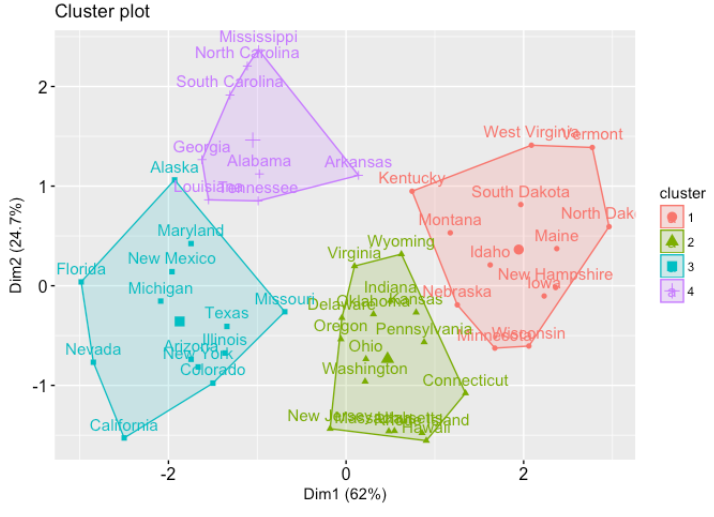
\includegraphics[width=0.6\textwidth]{../img/cluster-1.png}
    \caption{Ejemplo de clustering (Fuente: \cite{img-cluster-1}).}
\end{figure}

En la mayoría de las aplicaciones del AC se busca una partición de los datos en la que cada individuo u objeto pertenezca a un único cluster y el conjunto completo de clusters
contenga a todos los individuos. Sin embargo, esto no siempre es así y, de hecho, en algunas circunstancias, la superposición de clusters puede ofrecer una solución más aceptable.
Decimos que una respuesta aceptable del análisis cluster es que no se justifica la agrupación de los datos. El análisis cluster es un procedimiento objetivo; no están predefinidos,
sino que se forman a medida que avanza el análisis. \newline

Los datos básicos para la mayoría de las aplicaciones del análisis cluster se almacenan en una matriz $n \times p$, $X$, que contiene los valores de las variables que describen
cada objeto que se va a agrupar, es decir,

\[
X = [x_{ij}]_{i=1,\dots,n,\, j=1,\dots,p} =
\begin{bmatrix}
x_{11} & x_{12} & \cdots & x_{1p} \\
x_{21} & x_{22} & \cdots & x_{2p} \\
\vdots & \vdots & \ddots & \vdots \\
x_{n1} & x_{n2} & \cdots & x_{np}
\end{bmatrix}
\]
%       OBSERVA QUE ES LO CONTRARIO DE LO QUE DIJIMOS EN DATOS ÓMICOS (LA TRASPUESTA)?????? QUÉ HAGO?
donde $x_{ij}$ cuantifica la variable $j$ en la muestra $i$. El AC tratará de desarrollar un esquema de clasificación que particionará las filas de $X$ en $k$ clusters \cite{clustering-2}. %referencia: clustering-2.pdf


% medidas de proximidad (simularidad, disimilaridad)
\subsection{Medidas de proximidad}

%Para desarrollar esta sección se han utlizado las siguientes referencias bibliográficas:\cite{Bib-5}\cite{clustering-2}. \newline%clustering-2 %Bib-5 \newline

Dado que el análisis cluster trata de identificar los vectores que son similares y agruparlos en clusters, es esencial contar con herramientas que permitan evaluar la cercanía o 
distancia entre los objetos que se están agrupando: las \textit{medidas de proximidad}. Las decisiones sobre cómo se van a formar los clusters dependen directamente de las medidas de proximidad utilizadas, ya que estas 
definen cómo se calcula la similitud o diferencia entre los distintos elementos. \newline

Si una medida de proximidad representa \textit{similaridad}, el valor de la medida incrementa 
cuanto más similares sean dos objetos. Alternativamente, si la medida de proximidad representa \textit{disimilitud}, el valor de la medida disminuye a medida que dos objetos se vuelven más 
parecidos.

\subsubsection{Medidas de Disimilaridad}

Cuando todas las variables registradas son continuas, las proximidades entre los individuos generalmente se cuantifican mediante medidas de disimilaridad o medidas de distancia. 
Por ello, definiremos el concepto de \textit{disimilaridad} análogamente al de distancia.

\begin{definicion}
    Sean $\Omega \subset \mathbb{R}^{n}$ un conjunto de puntos de $\mathbb{R}^{n}$ y $x,y \in \Omega$ dos puntos cualesquiera de dicho conjunto. Entendemos por disimilaridad a toda 
    aplicación $d: \Omega \times \Omega \longrightarrow \mathbb{R}$ que satisface las siguientes propiedades:

    \begin{itemize}
        \item[i)] $d(x,y) \ge 0$
        \item[ii)] $d(x,y)= 0 \Longleftrightarrow x = y$
        \item[iii)] $d(x,y) = d(y,x)$ (simétrica)
    \end{itemize}
    Se dice que la disimilaridad es \textit{métrica} si satisface una cuarta propiedad:
    \begin{itemize}
        \item[iv)] $d(x,y) \leq d(x,z) + d(z,y) \forall z \in \Omega$, 
    \end{itemize}
        
    y se dirá \textit{ultramétrica} si es métrica y además cumple:
        
    \begin{itemize}
        \item[v)] $d(x,y) \leq \max\{d(x,z),d(y,z)\}$
    \end{itemize}
        
\end{definicion}

\vspace{0.2cm}
A continuación presentamos algunas de las medidas de disimilaridad más usadas. Hemos de hacer notar que estas medidas normalmente se usan para medir cuán próximos están los individuos, 
pero si se quiere medir entre variables, también son válidas. Simplemente habría que trasponer la matriz $X$ y trabajar con ella. \newline

Toda la información que sigue a partir de este punto, ha sido extraída de las fuentes bibliográficas:\cite{Bib-1, Bib-5, Bib-6, clustering-2, clustering-1}. \newline


Las medidas de disimilaridad se usan ante la necesidad de agrupar objetos con características similares. Una medida de disimilaridad adecuada es la distancia entre 
dos observaciones. Se considera una medida de disimilaridad por el hecho de que la distancia aumenta conforme dos individuos se alejan. \newline

Una gran variedad de distancias pueden generarse mediante la norma\footnote[10]{Norma: Una \textit{norma} en un espacio vectorial $X$ es una aplicación $\|\cdot\| \rightarrow \mathbb{R}$ que verifica:
\begin{itemize}
    \item[(N.1)] Desigualdad triangular: $\|x+y\| \leq \|x\| + \|y\| \forall x,y \in X$
    \item[(N.2)] Homogeneidad por homotecias: $\|\lambda x\| = |\lambda| \|x\| \forall x \in \mathbb{X}$, $\lambda \in \mathbb{R}$
    \item[(N.3)] No degeneración: $x \in X$, $\|x\| = 0 \Rightarrow x = 0$. \cite{def-norma}  
\end{itemize}.} $L_{r}$, $r \geq 1$, 

% definición norma: https://www.ugr.es/~rpaya/documentos/AnalisisI/2014-15/Normados.pdf

\[
d_{ij} = \|x_{i} - x_{j}\|_{r} = \{\sum_{k=1}^{p} |x_{ik}-x_{jk}|^{r}\}^{\frac{1}{r}} \hspace{2cm} (1)
\]

donde $x_{ik}$ denota el valor de la $k$-ésima variable en el objeto $i$. A esta distancia se la conoce por el nombre de \textit{distancia de Minkowsi}\newline

En lo que sigue, consideremos $x_{i}, x_{j} \in \mathbb{R}^{p}$ dos individuos de la población. Esto es, dos filas de la matriz $X$ que contine los datos. 
Definimos las siguientes medidas de disimilaridad:

\begin{definicion}

Definimos la \textit{distancia euclídea} como la derivada de la norma $L_{2}$ (caso particular de la distancia de Minkowski cuando $r=2$), 

\[
d_{2}(x_{i},x_{j}) = \|x_{i} - x_{j}\|_{2} = \sqrt{(x_{i}-x_{j})^{'}(x_{i}-x_{j})} = \sqrt{\sum_{j=1}^{p}(x_{j}-y_{j})^{2}}
\] 

\end{definicion}


De entre todas las medidas de disimilaridad, y de todas las métricas de Minkowski, la distancia Euclidea es la más común. Hemos de tener en cuenta que la 
distancia euclidea (y la euclidea al cuadrado) suelen calcularse a partir de datos en bruto, 
no de datos estandarizados. Esto presenta varias ventajas (p. ej., la distancia entre dos objetos cualesquiera no se ve afectada por la adición de nuevos objetos 
al análisis, que podrían ser valores atípicos). Sin embargo, las distancias pueden verse considerablemente afectadas por las diferencias de escala entre las 
dimensiones a partir de las cuales se calculan.  Por ejemplo, si una de las dimensiones representa una longitud medida en centímetros y luego se convierte a milímetros (multiplicando los 
valores por 10), las distancias euclidianas o euclidianas al cuadrado resultantes (calculadas a partir de múltiples dimensiones) pueden verse considerablemente 
afectadas y, en consecuencia, los resultados de los análisis de conglomerados pueden ser muy diferentes. \newline


\begin{observacion}
La \textit{distancia euclidea al cuadrado} puede resultar útil para asignar progresivamente mayor importancia a los objetos más separados. Además, al evitar las
raíces cuadradas, los cálculos se simplifican.
\end{observacion}


\begin{definicion}

    Se denomina distancia \textit{Manhattan}, \textit{City Block}, \textit{Hamming}, o \textit{$d_{1}$}, a la distancia derivada de la norma $L_{1}$, que viene dada por
    
    \[
    d_{1}(x_{i},x_{j}) = \sum_{k=1}^{p} |x_{ik}-x_{jk}|
    \]
    
\end{definicion}

Se utiliza cuando todas las características (variables) son binarias y mide el número de características en las que dos individuos difieren.

\begin{definicion}  % referencia: https://en.wikipedia.org/wiki/Lp_space
    
    Tomando límite cuando $r \rightarrow \infty$, la distancia derivada del límite de la norma $L_{r}$, llamada \textit{norma del máximo}, $L_{\infty}$, es la que se conoce
    como \textit{distancia de Chebychev}, y viene dada por

    \[
    d_{\infty}(x_{i},x_{j}) = \max_{k=1,\dots,p} |x_{ik}-x_{jk}|
    \]
\end{definicion}

\begin{observacion}
    La distancia euclidea la podemos ver como un caso particular de la distancia:
    \[
    d_{M}(x_{i},x_{j}) = \sqrt{(x_{i}-x_{j})^{'}M(x_{i}-x_{j})}
    \]

    cuando $M=I_{p}$, la matriz identidad de orden $p$.
\end{observacion}

Supongamos que $M$ es la matriz de covarianzas de las variables (las columnas de la matrix $X$ de datos), que se define de la siguiente forma:

\[
M=\Sigma = \frac{1}{p} \sum_{i=1}^{n}(x_{ij}-\overline{x}_{j})(x_{ij}-\overline{x}_{j})^{'}, \hspace{0.2cm} j=1,...,p 
\]

Podemos observar que si $p \geq n$, la matriz de covarianzas $\Sigma$, es definida positiva y, por consiguiente, es invertible. Esto nos permite 
definir la siguiente medida de disimilaridad:

\begin{definicion}
    Definimos la \textit{distancia de Mahalanobis} para individuos, como:
    \[
    D_{\Sigma}(x_{i},x_{j}) = \sqrt{(x_{i}-x_{j})^{'}\Sigma^{-1}(x_{i}-x_{j})}
    \]
\end{definicion}

A diferencia de la distancia Euclidea, la de Mahalanobis es invariante frente a cambios de escala. En efecto, sea $C_{n\times n}$ una matriz no singular
de orden $n$, entonces:

\[
D_{\Sigma}(Cx_{i},Cx_{j}) = \sqrt{(Cx_{i},Cx_{j})^{'}[\frac{1}{p}C(x_{ij}-\overline{x}_{j})(x_{ij}-\overline{x}_{j})^{'}C^{'}]^{-1}(Cx_{i},Cx_{j})} = 
\]
\[
= \sqrt{(x_{i},x_{j})^{'}C^{'}(C^{'})^{-1}[\frac{1}{p}(x_{ij}-\overline{x}_{j})(x_{ij}-\overline{x}_{j})^{'}]^{-1}C^{-1}C(x_{i},x_{j})} = 
\]    
\[
= \sqrt{(x_{i}-x_{j})^{'}\Sigma^{-1}(x_{i}-x_{j})} = D_{\Sigma}(x_{i},x_{j})
\]

La distancia de Mahalanobis no se usa comúnmente en técnicas de clustering porque calcula la matriz $\Sigma$ considerando todos los individuos juntos, en lugar 
de tratar los objetos de cada clúster por separado. Además, su cálculo es más complejo que el de otras métricas. Sin embargo, puede aplicarse dentro de 
cada clúster en una fase específica del proceso \cite{cluster-mahalanobis}.


\subsubsection{Medidas de similaridad}

Como en la subsección anterior, consideremos $x_{i},x_{j}$ dos vectores cualesquiera de $\mathbb{R}^{p}$. \newline

\begin{definicion}
Sea $\Omega \subset{\mathbb{R}^{n}}$ un conjunto de puntos de $\mathbb{R^{p}}$. Llamaremos \textit{similaridad} a toda aplicación $s:\Omega \times \Omega \rightarrow \mathbb{R}$
que satisfaga las siguiente propiedades:

\begin{itemize}
    \item[i)] $0 \leq s(x_{i},x_{j}) \leq 1$
    \item[ii)]$s(x_{i},x_{j}) = 1$ si y solo si $x_{i} = x_{j}$
    \item[iii)] $s(x_{i},x_{j}) = s(x_{j},x_{i})$ (simétrica)
\end{itemize}
\end{definicion}

Las condiciones $(i)$ y $(ii)$ aseguran que toda similaridad es siempre positiva e identicamente $1$ cuando los objetos $i$ y $j$ sean iguales. \newline

\begin{observacion}
    Podemos formar una disimilaridad a partir de una similaridad, sin más que hacer:
    \[
    d_{ij} = 1 - s_{ij}
    \]
    u otra función decreciente. Sin embargo, a diferencia de las disimilaridades, no constituye una métrica. \newline
    Naturalmente, podríamos pensar si esto también ocurre a la inversa, es decir, si dada una medida de disimilaridad $d_{ij}$, podemos construir una medida de similaridad, sin más que 
    despejar $s_{ij}$ en la anterior expresión: 
    \[
    s_{ij} = 1/(1+d_{ij})
    \]
    Pero como $d_{ij}$ no está acotada superiormente, $s_{ij} \in (0,1]$, lo cual implica que $s_{ij} \neq 0$. Es por ello que no se pueden crear similaridades a partir de
    disimilaridades.
\end{observacion}

A continuación presentamos las principales medidas de similaridad que se usan en el ámbito del análisis cluster. \newline

\begin{definicion}
Definimos el \textit{coeficiente de correlación de Pearson} entre los objetos $x_{i},x_{j}$, como
\[
q_{ij} = \frac{\sum_{k=1}^{p}(x_{ik}-\overline{x}_{i.})(x_{jk}-\overline{x}_{j.})}{\left[\sum_{k=1}^{p}(x_{ik}-\overline{x}_{i.})^{2}\sum_{k=1}^{p}(x_{jk}-\overline{x}_{j.})^{2} \right]}
\]   
\end{definicion}

donde $\overline{x}_{i.} = \sum_{k=1}^{p}\frac{x_{ik}}{p}$ y $\overline{x}_{j.} = \sum_{k=1}^{p}\frac{x_{jk}}{p}$. \newline

\begin{observacion}
    Dado que $q_{ij} \in [-1,1]$, es claro que no satisface la primera condición necesaria para ser una similaridad. No obstante, esto cambia si consideramos en su lugar, el 
    valor absoluto del mismo, $|q_{ij}|$, o bien tomando $1-q_{ij}^{2}$. 
\end{observacion}

Presentamos ahora otra medida de similaridad para las filas de $X$.

\begin{definicion}
    Definimos el \textit{coseno del ángulo $\theta$} entre los vectores $x_{i},x_{j}$ como
    \[
    cos \theta = c_{ij} = \frac{x_{i}^{'}x_{j}}{\|x_{i}\| \|x_{j}\|}
    \]
\end{definicion}

\begin{observacion}
    Podemos ver que estamos en la misma situación que antes, $c_{ij} \in [-1,1]$, lo cual indica que no verifica la propiedad $1$ de las medidas de similaridad. La solución a esto es 
    la misma que en el caso anterior: trabajar con $\|q_{ij}\|$ o $\|1-q_{ij}^{2}\|$. \newline
\end{observacion}

Llegados a este punto en el que ya sabemos medir cómo de diferentes o similares son los objetos que queremos agrupar, es el momento de 
introducir distintas estrategias o algoritmos de agrupación, que pueden ser jerárquicas o no jerárquicas. 

% clústering jerárquico

\subsection{Métodos jerárquicos}  % Bib-1, Bib-2, Bib-5, bejar-AC-2, gallardo-jerarquicos

La información recogida en esta subsección y en las sucesivas subsubsecciones se ha obtenido principalmente de las fuentes biliográficas \cite{Bib-1, Bib-5, bejar-AC, Bib-2, gallardo, bejar-AC-2}. \newline

Los \textit{métodos jerárquicos} para el análisis cluster representan un intento de encontrar buenos clusters en los datos mediante la combinación o división de clusters, con el propósito de
minimizar (maximizar) una medida de disimilaridad (similaridad). Hay dos tipos de métodos jerárquicos: los \textit{aglomerativos} y los \textit{disociativos}. Los aglomerativos comienzan 
con clusters que contienen un solo objeto y sucesivamente van combinando clusters hasta que todos forman un único cluster. Los disociativos, por su parte, hacen justo lo contrario: 
comienzan con todos los objetos agrupados en un único cluster, a continuación dividen dicho cluster en dos clusters separados, y así sucesivamente hasta formar clusters con un solo objeto. 

\begin{observacion}
Aunque se le suele prestar más atención a los métodos aglomerativos, los disociativos proporcionan clusterings más sofisticados y robustos.
\end{observacion}

\subsubsection{Dendrograma}

El resultado final de todo método jerárquico es lo que se conoce como \textit{dendograma} o \textit{diagrama en árbol jerárquico}. Es una representación gráfica del clústering que generalmente se
dibuja en sentido inverso, comenzando desde el último cluster que se ha formado y que engloba a todos los objetos. En el punto de similaridad donde dos clusters se combinan 
para dar lugar al cluster final, este se divide en dos clusters padres y así sucesivamente; la solución con $k$ clusters se obtiene fusionando algunos clusters de la solución con $(k+1)$. \newline

El dendrograma puede dibujarse horizontal o verticalmente, queda a elección de cada uno; ambas formas proporcionan la misma información. En nuestro caso, lo consideraremos en vertical. Nos permite 
determinar la altura del criterio de unión a la que los clusters se combinan para formar un nuevo cluster más grande. Los elementos similares se combinan a alturas bajas, mientras que los elementos
más disímiles se combinan a mayor altura en el dendrograma. Por lo tanto, es la diferencia de alturas la que define la proximidad de los individuos entre sí. Cuanto mayor sea la distancia entre las
alturas a las que se combinan los clusters, más fácilmente podremos identificar la estructura sustancial de los datos. \newline

Cortando el dendrograma a una altura adecuada, podremos obtener una partición de los datos en un número específico de grupos. Si dibujamos una línea horizontal a una altura adecuada, el número, $k$, de 
líneas verticales intersecadas por dicha línea horizontal determina una solución con $k$ clusters. Por tanto, estamos diciendo que cada intersección de la horizontal con una de las $k$ líneas verticales
representa un cluster y los elementos que están por debajo de dicha intersección serán los elementos que conforman el cluster. \newline

Nos podemos preguntar cómo saber a qué altura cortar el dendrograma. La respuesta es que depende; deberemos cortar a aquella altura que mejor represente los datos de entrada.\newline % bejar-AC-2

\begin{nota}
    
    Cabe remarcar que, si bien las distancias verticales son importantes a la hora de determinar una solución, las horizontales son totalmente irrelevantes. \newline

\end{nota}

\begin{ejemplo}

    Vemos qué información nos puede dar este dendrograma sobre el número de clusters, aproximado, en los que podríamos agrupar un conjunto de datos:

    \begin{figure}[h]
        \centering
        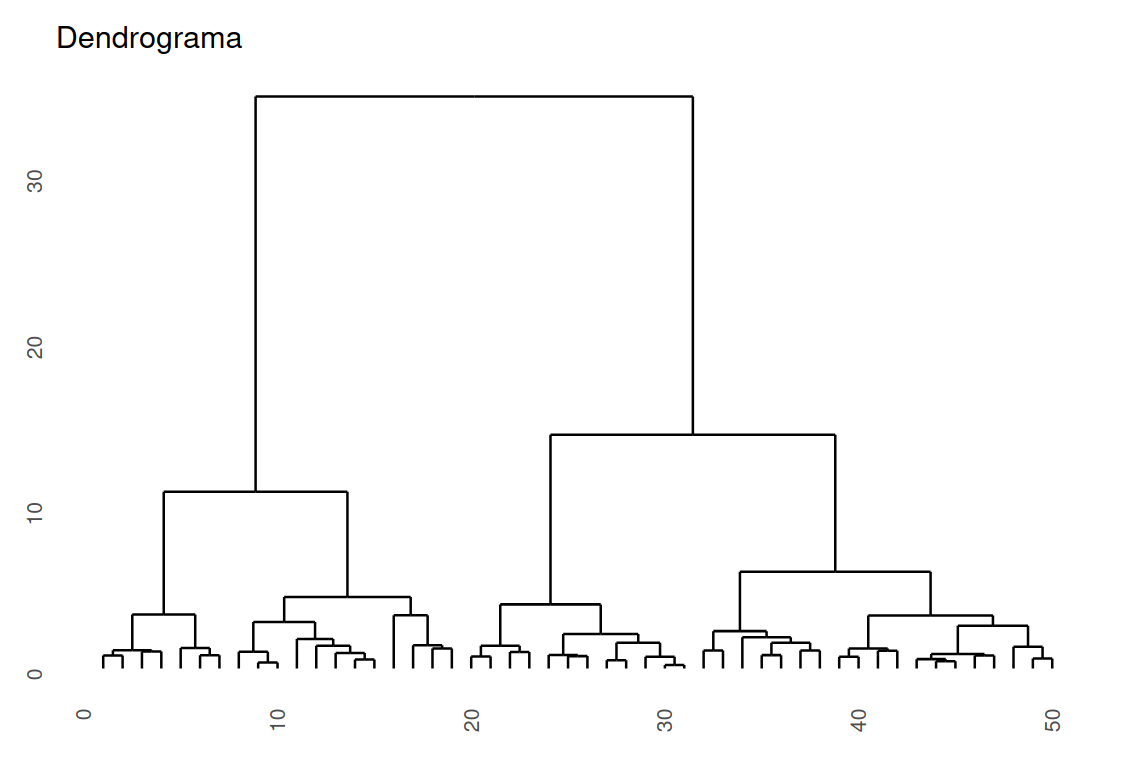
\includegraphics[width=0.5\textwidth]{../img/dendrograma-1.png}
        \caption{Ejemplo de dendrograma (Fuente: \cite{bejar-AC-2}).}
    \end{figure}

    \FloatBarrier

    Aclaremos que en el eje vertical tenemos la \textit{distancia euclidea} que existe entre cada grupo y en el eje horizontal, los datos. Las línea verticales son los
    agrupamientos que, a medida que vamos subiendo, van disminuyendo, hasta acabar en uno solo. Observamos que hay una gran separación entre las ramas en un entorno alrededor
    de $10$, por lo que, si trazáramos una línea horizontal a una altura por encima o por debajo de $10$, identificamos $3$ y $4$ clusters, respectivamente. \newline

    No podemos afirmar nada acerca del número de clusters óptimo con esta información. Habría que utilizar otros métodos, tanto visuales como matemáticos que nos permitan
    hacer una afirmación acerca de $k$ un poco más rotunda.

\end{ejemplo}


\subsubsection{Métodos jerárquicos aglomerativos}  %gallardo y Bib-5

A continuación, vamos a analizar los principales métodos jerárquicos aglomerativos. Hemos de aclarar que ninguno de los que presentaremos es más eficiente que otro. Esto 
dependerá de la naturaleza de los datos y el enfoque que tenga el análisis. \newline

\textbf{Estrategia de la distanca mínima o máxima similaridad} \newline

Del inglés \textit{single linkage}, traducido como \textit{encadenamiento simple}, y más conocida como la estrategia del \textit{vecino más cercano} es una estrategia que
se basa en combinar dos clusters que tengan distancia mínima (o máxima similaridad), siendo esta la distancia mínima entre sus componentes. \newline

Sean $C_{i}$ y $C_{j}$ dos clusters cualesquiera con $n_{i}$, $n_{j}$ elementos, respectivamente, y sean $x^{i}_{k} \in C_{i}$ , $x^{j}_{m} \in C_{j}$, con $k=1,\dots,n_{i}$, $m=1,\dots,n_{j}$ dos elementos de dichos clusters. La 
distancia entre $C_{i}$ y $C_{j}$ viene dada por

\[
d(C_{i},C_{j}) = \min_{\substack{k=1,\dots,n_{i} \\ m=1,\dots,n_{j}}}\{d(x^{i}_{k},x^{j}_{m}) \text{ | } x^{i}_{k} \in C_{i} \text{ y } x^{j}_{m} \in C_{j}\}
\]

donde $d(x^{i}_{k},x^{j}_{m})$ es la distancia Euclidea, generalmente, o cualquier otra distancia entre los elementos $x^{i}_{k},x^{j}_{k}$ de los clusters. 

Equivalentemente, en un contexto en el que usemos similaridad, se unirán dos clusters $C_{i}, C_{j}$ si

\[
s(C_{i},C_{j}) = \max_{\substack{k=1,\dots,n_{i} \\ m=1,\dots,n_{j}}}\{s(x^{i}_{k},x^{j}_{m}) \text{ | } x^{i}_{k} \in C_{i} \text{ y } x^{j}_{m} \in C_{j}\}
\]

\textbf{Estrategia de la distancia máxima o mínima similaridad}

Conocido también como el método del encadenamiento completo, al contrario que en la estrategia anterior, esta se basa en calcular la distancia máxima 
entre los clusters teniendo en cuenta la distancia máxima entre sus componentes. Esto es, ponemos el foco de atención en los elementos más dispares de 
los clusters, es decir, los que están a mayor distancia o son menos símiles. \newline

Sean entonces $C_{i}$ y $C_{j}$ dos clusters cualesquiera con $n_{i}$, $n_{j}$ elementos, respectivamente y sean $x^{i}_{k} \in C_{i}$ , $x^{j}_{m} \in C_{j}$, 
con $k=1,\dots,n_{i}$, $m=1,\dots,n_{j}$ dos elementos de dichos clusters. Entonces, la distancia entre dichos clusters viene dada por:

\[
d(C_{i},C_{j}) = \max_{\substack{k=1,\dots,n_{i} \\ m=1,\dots,n_{j}}}\{d(x^{i}_{k},x^{j}_{m}) \text{ | } x^{i}_{k} \in C_{i} \text{ y } x^{j}_{m} \in C_{j}\}
\]

Equivalentemente, si lo miramos desde el punto de vista de la similaridad, se unirán dos clusters $C_{i}, C_{j}$ si

\[
s(C_{i},C_{j}) = \min_{\substack{k=1,\dots,n_{i} \\ m=1,\dots,n_{j}}}\{s(x^{i}_{k},x^{j}_{m}) \text{ | } x^{i}_{k} \in C_{i} \text{ y } x^{j}_{m} \in C_{j}\}
\]

\textbf{Estrategia de la distancia o similitud promedio}

Mientras que en las dos estrategias anteriores la combinación de dos clusters en uno dependía únicamente de un único par de objetos dentro de cada cluster, 
y se usaba la distancia máxima o mínima, la estrategia de la distancia promedio calcula la distancia entre dos clusters como el promedio de las disimilaridades 
en cada cluster. Dependiendo de si consideramos el tamaño de los clusters en el promedio o no, podemos distinguir entre dos estrategias diferentes: la no ponderada
y la ponderada. \newline

Consideremos en lo que sigue dos clusters $C_{i}$, $C_{j}$ con $n_{i},n_{j}$ elementos, y $x^{i}_{k},x^{j}_{m}$ dos elementos de $C_{i},C_{j}$, respectivamente con $k=1,\dots,n_{i}$, $m=1,\dots,n_{j}$.

\begin{itemize}
    \item \textbf{No ponderada} \newline

    Supongamos, sin pérdida de generalidad, que $C_{i}$ está constituido por dos clusters $C_{i_{1}}$ y $C_{i_{2}}$ con $n_{i_{1}},n_{i_{2}}$ elementos respectivamente, la distancia entre $C_{i}$ y $C_{j}$ viene dada por
    \[
    d(C_{i},C_{j}) = \frac{d(C_{i_{1}}, C_{j}) + d(C_{i_{2}}, C_{j})}{2}
    \]

    Observamos que esta distancia es independiente de los tamaños de los clusters involucrados. Esto quiere decir que las distancias respecto a $C_{j}$ de $C_{i_{1}}$ y $C_{i_{2}}$
    tienen el mismo peso. 

    \item \textbf{Ponderada} \newline
    
    A diferencia de la anterior estrategia, esta distancia es el promedio ponderado de las distancias de las componentes del cluster con respecto a las del otro. Supongamos que 
    $C_{i}$ está constituido por dos clusters $C_{i_{1}}$, $C_{i_{2}}$ con $n_{i_{1}}$,$n_{i_{2}}$ elementos tales que $n_{i} = n_{i_{1}}+n_{i_{2}}$ y tomemos los elementos $x^{i_{1}}_{z} \in C_{i_{1}}$, $x^{i_{2}}_{w} \in C_{i_{2}}$, donde 
    $z = 1,\dots,n_{i_{1}} $ y $w = 1,\dots,n_{i_{2}}$. Entonces, la distancia promedio pondera entre $C_{i},C_{j}$ viene dada por
    
    \[
    d(C_{i},C_{j}) = \frac{\sum_{k=1}^{n_{i}}\sum_{m=1}^{n_{j}}d(x^{i}_{k},x^{j}_{m})}{n_{i}n_{j}} = \frac{1}{(n_{i_{1}}+n_{i_{2}})n_{j}} \sum_{k=1}^{n_{i_{1}}+n_{i_{2}}} \sum_{m=1}^{n_{j}} d(x^{i}_{k},x^{j}_{m}) = 
    \]
    \[
    = \frac{1}{(n_{i_{1}}+n_{i_{2}})n_{j}} \sum_{z=1}^{n_{i_{1}}} \sum_{m=1}^{n_{j}} d(x^{i_{1}}_{z},x^{j}_{m}) + \frac{1}{(n_{i_{1}}+n_{i_{2}})n_{j}} \sum_{w=1}^{n_{i_{2}}} \sum_{m=1}^{n_{j}} d(x^{i_{2}}_{w},x^{j}_{m}) = 
    \]
    \[
    = \frac{n_{i_{1}}}{(n_{i_{1}}+n_{i_{2}})n_{j}n_{i_{1}}} \sum_{z=1}^{n_{i_{1}}} \sum_{m=1}^{n_{j}} d(x^{i_{1}}_{z},x^{j}_{m}) + \frac{n_{i_{2}}}{(n_{i_{1}}+n_{i_{2}})n_{j}n_{i_{2}}} \sum_{w=1}^{n_{i_{2}}} \sum_{m=1}^{n_{j}} d(x^{i_{2}}_{w},x^{j}_{m}) = 
    \]
    \[
    = \frac{n_{i_{1}}}{n_{i_{1}}+n_{i_{2}}} d(C_{i_{1}},C_{j}) + \frac{n_{i_{2}}}{n_{i_{1}}+n_{i_{2}}} d(C_{i_{2}},C_{j}) = 
    \]
    \[
    = \frac{n_{i_{1}}d(C_{i_{1}},j) + n_{i_{2}}d(C_{i_{2}},C_{j})}{n_{i_{1}}+n_{i_{2}}}
    \]

\end{itemize}

\vspace{0.5cm}

\textbf{Método del centroide} \newline  % gallardo y Bib-5

En este método, para determinar cuán semejantes son dos clusters, vamos a poner el foco de atención en los \textit{centroides} de los mismos, es decir, en los vectores de medias de las variables 
observadas sobre los individuos que conforman el cluster. Entonces, los centroides de los clusters $C_{i},C_{j}$ son

\[
\bar{x}^{i} = \frac{\sum_{k=1}^{n_{i}}x^{i}_{k}}{n_{i}} = \begin{bmatrix} \bar{x}^{i}_{1} \\  \bar{x}^{i}_{2} \\ \vdots \\ \bar{x}^{i}_{n_{i}} \end{bmatrix} \text{ y } \bar{x}^{j} = \frac{\sum_{m=1}^{n_{j}}x^{j}_{m}}{n_{j}} = \begin{bmatrix} \bar{x}^{j}_{1} \\  \bar{x}^{j}_{2} \\ \vdots \\ \bar{x}^{j}_{n_{j}} \end{bmatrix} 
\]

respectivamente, y el cuadrado de la distancia Euclidea entre ambos centroides es $d^{2}(C_{i},C_{j}) = \|\bar{x}^{i} - \bar{x}^{j}\|^{2}$. Se persigue entonces el objetivo de encontrar clusters que hagan mínima la 
distancia entre sus centroides, para, consecuentemente, combinarlos en un nuevo cluster, que llamaremos $C_{t}$ con centroide $\bar{x}^{t} = \frac{(n_{i}\bar{x}^{i} + n_{j}\bar{x}^{j})}{n_{i}+n_{j}}$. Se calcularían 
de nuevo las distancias entre dicho centroide y el de los demás clusters. Continuaríamos el proceso hasta obtener un único cluster.\newline

El método del centroide se denomina \textit{método de la mediana} si se utiliza un promedio no ponderado de los centroides: $\bar{x}^{t} = \frac{(\bar{x}^{i} +\bar{x}^{j})}{2}$. Este método es preferible cuando $n_{i} >> n_{j}$ o
viceversa. \newline

Calculamos el cuadrado de la distancia Euclidea entre el cluster $C_{t}$ y el centroide $\bar{x}^{u}$ de un tercer cluster $C_{u}$ de la siguiente forma:
\[
d^{2}(C_{t}, C_{u}) = \left( \frac{n_{i}}{n_{i} + n_{j}} \right) d^{2}(C_{i},C_{j}) + \left (\frac{n_{j}}{n_{i} + n_{j}}\right) d^{2}(C_{i},C_{u}) - \left( \frac{n_{i}n_{j}}{n_{i} + n_{j}}\right) d^{2}(C_{i},C_{j})
\]

\vspace{0.5cm}

\textbf{Método de Ward} \newline

El \textit{método de Ward}, también conocido como \textit{método de la suma incremental de cuadrados}, es un método jerárquico aglomerativo cuya filosofía la podemos resumir de la siguiente forma: \newline

Supongamos que tenemos $m$ elementos que queremos agrupar. Comenzamos con $m$ clusters, cada uno de ellos con un único individuo. A continuación, estudiamos la similaridad de dichos clusters y, el par de clusters más
similares se combinan, reduciendose el número de clusters en uno. Se sigue este proceso hasta que todos los clusters estén fusionados. El objetivo de este método es, en definitiva, encontrar en cada iteración, los dos 
clusters tales que su fusión genere el menor incremento en el valor total de la suma de los cuadrados de las diferencias entre cada elemento y el centroide del cluster. \newline

Para desarrollar formalmente el método, vamos a establecer la siguiente notación:

\begin{itemize}
    \item Notaremos por $x^{k}_{ij}$ al valor de la $j$-ésima variable observada sobre el $i$-ésimo individuo dentro del $k$-ésimo cluster. Suponemos que dicho cluster estará formado por $n_{k}$ indivduos.
    \item Al centroide del $k$-ésimo cluster lo denotaremos como hicimos en el método del centroide: $m^{k}$, con $n$ componentes, $m^{k}_{j}$.
    \item $E_{k}$ será la suma de los cuadrados de las distancias (distancia euclidea) de cada individuo del cluster $k$ al centroide (los errores del cluster $k$). Esto es,
    \[
    E_{k} = \sum_{i=1}^{n_{k}}\sum_{j=1}^{n}(x^{k}_{ij} - m^{k}_{j})^{2} = \sum_{i=1}^{n_{k}}\sum_{j=1}^{n}(x^{k}_{ij})^{2} - n_{k}\sum_{j=1}^{n}(m^{k}_{j})^{2}
    \]
    \item Llamaremos $E$ a la suma de los cuadrados de los errores de todos los clusters en su conjunto. Es decir, suponiendo que hubiera $h$ clusters
    \[
    E = \sum_{k=1}^{h} E_{k}
    \]
\end{itemize}


\begin{observacion}
    Notemos que al principio del método, $E_{k} = 0$, $\forall k \in \{1,\dots,m\}$ pues hay $m$ clusters compuestos por un solo individuo. \newline
    En cada etapa, buscaremos los dos clusters cuya fusión minimice el incremento en $E$.
\end{observacion}

Supongamos que en la siguiente etapa son $C_{p}$ y $C_{q}$ los dos clusters que se fusionan en uno nuevo, $C_{t}$. Entonces, el incremento de $E$, $\Delta E_{pq}$, vendrá dado por
\[
\Delta E_{pq} = E_{t} - E_{p} - E_{q} =
\]
\[
= \left[ \sum_{i=1}^{n_{t}}\sum_{j=1}^{n}(x^{t}_{ij})^{2} - n_{t}\sum_{j=1}^{n}(m^{p})^{2} \right] - \left[ \sum_{i=1}^{n_{k}}\sum_{j=1}^{n}(x^{p}_{ij})^{2} - n_{p}\sum_{j=1}^{n}(m^{p})^{2} \right] - \left[ \sum_{i=1}^{n_{q}}\sum_{j=1}^{n}(x^{q}_{ij})^{2} - n_{p}\sum_{j=1}^{n}(m^{q})^{2} \right] = 
\]
\[
\overset{n_{t} = n_{p}+n_{q}}{=} n_{p}\sum_{j=1}^{n}(m^{p}_{j})^{2} + n_{q}\sum_{j=1}^{n}(m^{q}_{j})^{2} - n_{t}\sum_{j=1}^{n}(m^{t}_{j})^{2}
\]

Ahora, por un lado sabemos por el apartado anterior que el centroide de un cluster $C_{c}$ se calcula como 
\[
m^{c} = \frac{\sum_{j=1}^{n_{c}}x^{c}_{j}}{n_{c}}
\]

Aplicando esto al cluster $C_{p}$, tenemos:
\[
m^{p} = \frac{\sum_{j=1}^{n_{p}}x^{p}_{j}}{n_{p}} \Longleftrightarrow n_{p}m^{p} = \sum_{j=1}^{n_{p}}x^{p}_{j}
\]

Para el cluster $C_{q}$:
\[
m^{q} = \frac{\sum_{j=1}^{n_{q}}x^{q}_{j}}{n_{q}} \Longleftrightarrow n_{q}m^{q} = \sum_{j=1}^{n_{q}}x^{q}_{j}
\]

Cuando fusionamos los clusters $C_{p}$ y $C_{q}$, tenemos un cluster $C_{t}$ de $n_{t} = n_{p} + n_{q}$ elementos, con centroide
\[
m^{t} = \frac{\sum_{j=1}^{n_{t}}x^{t}_{j}}{n_{t}}
\]

Como $C_{t}$ tiene todos los puntos de $C_{p}$ y $C_{q}$, podemos escribir
\[
\sum_{j=1}^{n_{t}}x^{t}_{j} = \sum_{j=1}^{n_{p}}x^{p}_{j} + \sum_{j=1}^{n_{q}}x^{q}_{j}
\]

Por lo que, si sustituimos en las expresiones de $n_{p}m^{p}$ y $n_{q}m^{q}_{j}$:
\[
\sum_{j=1}^{n_{t}}x^{t}_{j}  = n_{p}m^{p} + n_{q}m^{q}
\]

Multiplicando por $n_{t}$, obtenemos:
\[
n_{t}m^{t} = n_{p}m^{p} + n_{q}m^{q}
\]

Como esto es una igualdad vectorial, la igualdad se verifica componente a componente:

\[
n_{t}m^{t}_{j} = n_{p}m^{p}_{j} + n_{q}m^{q}_{j} \text{ con } j = 1,\dots,n
\]

Partiendo entonces de la igualdad $n_{t}m^{t}_{j} = n_{p}m^{p}_{j} + n_{q}m^{q}_{j}$, elevando al cuadrado ambos miembros obtenemos
\[
n_{t}^{2}(m^{t}_{j})^{2} = n^{2}_{p}(m^{p}_{j})^2 + n^{2}_{q}(m^{q}_{j})^{2} + 2n_{p}n_{q}m^{p}_{j}m^{q}_{j} = 
\]
\[
= n^{2}_{p}(m^{p}_{j})^2 + n^{2}_{q}(m^{q}_{j})^{2} + n_{p}n_{q}(2m_{j}^{p}m_{j}^{q}) = n^{2}_{p}(m^{p}_{j})^2 + n^{2}_{q}(m^{q}_{j})^{2} + n_{p}n_{q}((m_{j}^{p})^{2} + (m_{j}^{q})^{2} - (m^{p}_{j}-m^{q}_{j})^{2})
\]

de donde se obtiene
\[
n_{t}^{2}(m^{t}_{j})^{2} = n_{p}(n_{p}+n_{q})(m^{p}_{j})^{2} + n_{q}(n_{p}+n_{q})(m^{q}_{j})^{2} - n_{p}n_{q}(m_{j}^{p}-m_{j}^{q})^{2}
\]

Dividiendo por $n_{t}^{2}$ se obtiene
\[
(m_{j}^{t})^{2} = \frac{n_{p}}{n_{t}}(m^{p}_{j})^{2} + \frac{n_{q}}{n_{t}}(m_{j}^{q})^{2} - \frac{n_{p}n_{q}}{n_{t}^{2}}(m^{p}_{j}-m^{q}_{j})^{2}
\]

Por tanto, si sustituimos esta expresión en la del incremento, $\Delta E_{pq}$, nos queda lo siguiente:
\[
\Delta E_{pq} = n_{p}\sum_{j=1}^{n}(m^{p}_{j})^{2} + n_{q}\sum_{j=1}^{n}(m^{q}_{j})^{2} - n_{t}\sum_{j=1}^{n} \left[\frac{n_{p}}{n_{t}}(m^{p}_{j})^{2} + \frac{n_{q}}{n_{t}}(m_{j}^{q})^{2} - \frac{n_{p}n_{q}}{n_{t}^{2}}(m^{p}_{j}-m^{q}_{j})^{2}\right] \Longleftrightarrow
\]
\[
\Longleftrightarrow \Delta E_{pq} = n_{p}\sum_{j=1}^{n}(m^{p}_{j})^{2} + n_{q}\sum_{j=1}^{n}(m^{q}_{j})^{2} - m_{p}\sum_{j=1}^{n}(m_{j}^{p})^{2} - n_{q}\sum_{j=1}^{n}(m^{q}_{j})^{2} + \frac{n_{p}n_{q}}{n_{t}}\sum_{j=1}^{n}(m^{p}_{j}-m^{q}_{j})^{2}
\]
\vspace{0.5cm}
\[
\Rightarrow \Delta E_{pq} = \frac{n_{p}n_{q}}{n_{t}}\sum_{j=1}^{n}(m^{p}_{j}-m^{q}_{j})^{2}
\]

Obtenemos por consiguiente que el menor incremento de los errores cuadráticos es proporcional al cuadrado de la distancia euclidea de los centroides de los clusters fusionados. \newline

Veamos cómo calcular los incrementos a partir de otros ya previamente calculados. \newline
Sea $C_{t}$ el cluster que resulta de fusionar $C_{p}$ y $C_{q}$ y consideremos ahora otro cluster $C_{r}$ distinto a los demás. Entonces, por lo visto anteriormente, 
el incremento en $E$ que se produce al fusionar $C_{r}$ con $C_{t}$, viene dado por
\[
\Delta E_{rt} = \frac{n_{r}n_{t}}{n_{r}+n_{t}}\sum_{j=1}^{n}(m^{r}_{j}-m^{t}_{j})^{2}
\]

Como $n_{t}m^{t} = n_{p}m^{p} + n_{q}m^{q}$ y $n_{t} = n_{p}+n_{q}$, y sabemos también que $(m_{j}^{t})^{2} = \frac{n_{p}}{n_{t}}(m^{p}_{j})^{2} + \frac{n_{q}}{n_{t}}(m_{j}^{q})^{2} - \frac{n_{p}n_{q}}{n_{t}^{2}}(m^{p}_{j}-m^{q}_{j})^{2}$, deducimos que
\[
(m^{r}_{j}-m^{t}_{j})^{2} = (m^{r}_{j})^{2} + (m^{t}_{j})^{2} - 2m_{j}^{r}m_{j}^{t} = 
\]
\[
= (m_{j}^{r})^{2} + \frac{n_{p}}{n_{t}}(m^{p}_{j})^{2} + \frac{n_{q}}{n_{t}}(m^{q}_{j})^{2} - \frac{n_{p}n_{q}}{n_{t}^{2}}(m^{p}_{j}-m^{q}_{j})^{2} - 2m^{r}_{j}\frac{n_{p}m^{p}_{j} + n_{q}m^{q}_{j}}{n_{t}} = 
\]
\[
= \frac{n_{p}(m_{j}^{r})^{2}+n_{q}(m_{j}^{q})^{2}}{n_{t}} + \frac{n_{p}}{n_{t}}(m^{p}_{j})^{2} + \frac{n_{q}}{n_{t}}(m^{q}_{j})^{2} - \frac{n_{p}n_{q}}{n^{2}_{t}}(m^{p}_{j}-m^{q}_{j})^{2} - 2m^{r}_{j}\frac{n_{p}m^{p}_{j} + n_{q}m^{q}_{j}}{n_{t}} = 
\]
\[
= \frac{n_{p}}{n_{t}}(m^{r}_{j} - m^{p}_{j})^{2} + \frac{n_{q}}{n_{t}}(m^{r}_{j} - m^{q}_{j})^{2} - \frac{n_{p}n_{q}}{n_{t}^{2}}(m^{p}_{j}-m^{q}_{j})^{2}
\]

Obtenemos por tanto,

\[
\Delta E_{rt} = \frac{n_{r}n_{t}}{n_{r}+n_{t}} \sum_{j=1}^{n} (m^{r}_{j}-m^{t}_{j})^{2} = 
\]
\[
= \frac{n_{r}n_{t}}{n_{r}+n_{t}}\sum_{j=1}^{n} \left[\frac{n_{p}}{n_{t}}(m^{r}_{j} - m^{p}_{j})^{2} + \frac{n_{q}}{n_{t}}(m^{r}_{j} - m^{q}_{j})^{2} - \frac{n_{p}n_{q}}{n_{t}^{2}}(m^{p}_{j}-m^{q}_{j})^{2}\right] = 
\]
\[
= \frac{n_{r}n_{p}}{n_{r}+n_{t}}\sum_{j=1}^{n} (m^{r}_{j} - m^{p}_{j})^{2} + \frac{n_{q}n_{r}}{n_{r}+n_{t}}\sum_{j=1}^{n}(m^{r}_{j} - m^{q}_{j})^{2} - \frac{n_{r}n_{p}n_{q}}{n_{t}(n_{r}+n_{t})}(m^{p}_{j}-m^{q}_{j})^{2} = 
\]
\[
= \frac{1}{n_{r}+n_{t}}\sum_{j=1}^{n}\left[n_{r}n_{p}(m^{r}_{j}-m^{p}_{j})^{2} + n_{r}n_{q}(m^{r}_{j}-m^{q}_{j})^{2} - \frac{n_{r}n_{p}n_{q}}{n_{p}+n_{q}}(m^{p}_{j}-m^{q}_{j})^{2}\right] =
\]
\[
= \frac{1}{n_{r}+n_{t}}[(n_{r}+n_{p})\Delta E_{rp} + (n_{r}+n_{q})\Delta E_{rq} - n_{r}\Delta E_{pq}]
\]

\vspace{0.5cm}

\begin{nota}
    Se puede demostrar que esta relación no depende de la forma específica en que se mide la distancia, siempre que esta se defina a partir de 
    una norma inducida por un producto escalar o que satisfaga la ley del paralelogramo.
\end{nota}

\vspace{0.5cm}

Ofrecemos a continuación un pequeño ejemplo de aplicación de este método aglomerativo, de elaboración propia aunque basado en la fuente bibliográfica \cite{bejar-AC}.

\begin{ejemplo}

    Consideremos los siguientes datos de $5$ genotipos sobre los que se observan dos variables $X_{1}$ y $X_{2}$.

    \begin{table}[h]
        \centering
        \begin{tabular}{|c|c|c|}
            \hline
            \textbf{Genotipo} & \textbf{$X_{1}$} & \textbf{$X_{2}$} \\
            \hline
            $G_{1}$ & 7 & 10 \\
            \hline
            $G_{2}$ & 8 & 10 \\
            \hline
            $G_{3}$ & 6 & 5 \\
            \hline
            $G_{4}$ & 3 & 2 \\
            \hline
            $G_{5}$ & 11 & 10 \\
            \hline
            
        \end{tabular}
        \caption{Ejemplo método de Ward}

    \end{table}
    
    En la primera iteración del método, contamos con $5$ clusters, cada uno compuesto por un único punto (cada punto de nuestro dataset 
    en un cluster):

    \begin{table}[h]
        \centering
        \begin{tabular}{|c|c|c|c|c|}
            \hline
            \textbf{Partición} & \textbf{Centroides} & \textbf{$E_{k}$} & \textbf{$E$} & \textbf{$\Delta E$} \\
            \hline
            $G_{1},G_{2},G_{3},G_{4},G_{5}$ & los propios puntos & $E_{G_{1}} = E_{G_{2}}=E_{G_{3}}=E_{G_{4}}=E_{G_{5}}=0$ & $0$ & $0$ \\
            \hline
        \end{tabular}
        \caption{Nivel 0} 

    \end{table}

    A continuación, barajamos todas las parejas que podemos formar con estos $5$ elementos, para estudiar qué pareja de clusters generaría el menor
    $\Delta E$ al fusionarse. Estudiemos entonces las $\binom{5}{2} = 10$ combinaciones posibles.

    \begin{table}[h]
        \small
        \centering
        \begin{tabular}{| c | c | c | c | c |}
            \hline
            \textbf{Partición} & \textbf{Centroides} & \(E_{k}\) & \(E\) & \(\Delta E\) \\
            \hline
            (\(G_{1}, G_{2}\)), \(G_{3}, G_{4}, G_{5}\) & \(C_{G_{1}G_{2}} = (7.5, 10)\) & \(E_{G_{1}G_{2}} = 0.5\) & 0.5 & 0.5 \\
            \hline
            (\(G_{1}, G_{3}\)), \(G_{2}, G_{4}, G_{5}\) & \(C_{G_{1}G_{3}} = (6.5, 7.5)\) & \(E_{G_{1}G_{3}} = 13\) & 13 & 13 \\
            \hline
            (\(G_{1}, G_{4}\)), \(G_{2}, G_{3}, G_{5}\) & \(C_{G_{1}G_{4}} = (5, 6)\) & \(E_{G_{1}G_{4}} = 40\) & 40 & 40 \\
            \hline
            (\(G_{1}, G_{5}\)), \(G_{2}, G_{3}, G_{4}\) & \(C_{G_{1}G_{5}} = (9, 10)\) & \(E_{G_{1}G_{5}} = 8\) & 8 & 8 \\
            \hline
            (\(G_{2}, G_{3}\)), \(G_{1}, G_{4}, G_{5}\) & \(C_{G_{2}G_{3}} = (7, 7.5)\) & \(E_{G_{2}G_{3}} = 14.5\) & 14.5 & 14.5 \\
            \hline
            (\(G_{2}, G_{4}\)), \(G_{1}, G_{3}, G_{5}\) & \(C_{G_{2}G_{4}} = (5.5, 6)\) & \(E_{G_{2}G_{4}} = 44.5\) & 44.5 & 44.5 \\
            \hline
            (\(G_{2}, G_{5}\)), \(G_{1}, G_{3}, G_{4}\) & \(C_{G_{2}G_{5}} = (9.5, 10)\) & \(E_{G_{2}G_{5}} = 4.5\) & 4.5 & 4.5 \\
            \hline
            (\(G_{3}, G_{4}\)), \(G_{1}, G_{2}, G_{5}\) & \(C_{G_{3}G_{4}} = (4.5, 3.5)\) & \(E_{G_{3}G_{4}} = 9\) & 9 & 9 \\
            \hline
            (\(G_{3}, G_{5}\)), \(G_{1}, G_{2}, G_{4}\) & \(C_{G_{3}G_{5}} = (8.5, 7.5)\) & \(E_{G_{3}G_{5}} = 25\) & 25 & 25 \\
            \hline
            (\(G_{4}, G_{5}\)), \(G_{1}, G_{2}, G_{3}\) & \(C_{G_{4}G_{5}} = (7, 6)\) & \(E_{G_{4}G_{5}} = 64\) & 64 & 64 \\
            \hline
        \end{tabular}
        \caption{Nivel 1}
        
    \end{table}

    Observamos que se han de fusonar los elementos $G_{1}$ y $G_{2}$. En este nivel, la configuración de clusters es $(G_{1},G_{2}),G_{3},G_{4},G_{5}$. \newline

    A continuación, calculemos los incrementos que daría lugar las $\binom{4}{2} = 6$ posibles combinaciones.


    \begin{table}[h]
        \centering
        \begin{tabular}{|c|c|c|c|c|}
            \hline
            \textbf{Partición} & \textbf{Centroides} & \textbf{$E_k$} & \textbf{$E$} & \textbf{$\Delta E$} \\
            \hline
            ($G_{1},G_{2}, G_{3}$), $G_{4}, G_{5}$ & $C_{G_{1}G_{2}G_{3}} = (7, 8.33)$ & \makecell{$E_{G_{1}G_{2}G_{3}} = 18.67$ \\ $E_{G_{4}}=E_{G_{5}}=0$} & 18.67 & 18.17 \\
            \hline
            ($G_{1},G_{2}, G_{4}$), $G_{3}, G_{5}$ & $C_{G_{1}G_{2}G_{4}} = (6, 7.33)$ & \makecell{$E_{G_{1}G_{2}G_{4}} = 56.67$ \\ $E_{G_{3}}= E_{G_{5}}=0$} & 56.67 & 56.17 \\
            \hline
            ($G_{1},G_{2}, G_{5}$), $G_{3}, G_{4}$ & $C_{G_{1}G_{2}G_{5}} = (8.67, 10)$ & \makecell{$E_{G_{1}G_{2}G_{5}} = 8.67$ \\ $E_{G_{3}}= E_{G_{4}}=0$} & 8.67 & 8.17 \\
            \hline
            ($G_{3}, G_{4}$), ($G_{1},G_{2}), G_{5}$ & \makecell{$C_{G_{3}G_{4}} = (4.5, 3.5)$ \\ $C_{G_{1}G_{2}} = (7.5, 10)$} & \makecell{$E_{G_{3}G_{4}} = 9$ \\ $E_{G_{1}G_{2}} = 0.5$,$E_{G_{5}}=0$} & 9 & 8.5 \\  
            \hline
            ($G_{3}, G_{5}$), ($G_{1}G_{2}), G_{4}$ & $C_{G_{3}G_{5}} = (8.5, 7.5)$ & \makecell{$E_{G_{3}G_{5}}= 25$ \\ $E_{G_{1}G_{2}} = 0.5$, $E_{G_{4}}=0$} & 25.5 & 25 \\
            \hline
            ($G_{4}, G_{5}$), ($G_{1}G_{2}), G_{3}$ & $C_{G_{4}G_{5}} = (7, 6)$ & \makecell{$E_{G_{4}G_5} = 64$ \\ $E_{G_{1}G_{2}} = 0.5$, $E_{G_{3}}=0$} & 64.5 & 64 \\
            \hline
        \end{tabular}
        \caption{Nivel 2}
    \end{table}


    Inferimos de esta iteración que el genotipo $G_{5}$ deberá fusionarse con $G_{1}$ y $G_{2}$. De esta forma, nos queda la siguiente configuración: $(G_{1},G_{2}, G_{5}$), $G_{3}, G_{4}$. \newline

    Consideremos entonces las $\binom{3}{2} = 3$ posibles combinaciones que podemos hacer con los elementos de la configuración que se nos ha quedado:

    \begin{table}[h]
        \centering
        \begin{tabular}{|c|c|c|c|c|}
            \hline
            \textbf{Partición} & \textbf{Centroides} & \textbf{$E_k$} & \textbf{$E$} & \textbf{$\Delta E$} \\
            \hline
            ($G_{1},G_{2}, G_{5},G_{3})$, $G_{4}$ & $C_{G_{1}G_{2}G_{3}G_{5}} = (8,8.75)$ & \makecell{$E_{G_{1}G_{2}G_{3}G_{5}} = 32.75$ \\ $E_{G_{4}}=0$} & 32.75 & 24.08 \\
            \hline
            ($G_{1},G_{2}, G_{5},G_{4}$), $G_{3}$ & $C_{G_{1}G_{2}G_{4}G_{5}} = (7.25,8)$ & \makecell{$E_{G_{1}G_{2}G_{4}G_{5}} = 80.75$ \\ $E_{G_{3}}=0$} & 80.75 & 72.08 \\
            \hline
            ($G_{1},G_{2}, G_{5}$), ($G_{3}, G_{4}$) & \makecell{$C_{G_{1}G_{2}G_{5}} = (8.67,10)$ \\ $C_{G_{3}G_{4}} = (4.5,3.5)$} & \makecell{$E_{G_{1}G_{2}G_{5}} = 8.67$ \\ $E_{G_{3}G_{4}}=9$} & 17.67 & 9 \\
            \hline
            
        \end{tabular}
        \caption{Nivel 3}
    \end{table}

    Observamos que los elementos $G_{3}$ y $G_{4}$ se han de combinar en un cluster independiente. Es por ello que en este nivel la configuración de clusters que resulta es ($G_{1},G_{2}, G_{5}$), ($G_{3}, G_{4}$).\newline

    En la siguiente iteración, la única posibilidad es que todos los elementos estén en un único cluster: ($G_{1},G_{2}, G_{5},G_{3}, G_{4}$):

    \begin{table}[h]
        \centering
        \begin{tabular}{|c|c|c|c|c|}
            \hline
            \textbf{Partición} & \textbf{Centroides} & \textbf{$E_{k}$} & \textbf{$E$} & \textbf{$\Delta E$} \\
            \hline
            $(G_{1},G_{2},G_{3},G_{4},G_{5})$ & $C_{G_{1}G_{2}G_{3}G_{4}G_{5}}=(7,7.4)$ & $E_{G_{1}G_{2}G_{3}G_{4}G_{5}}=89.2$ & $89.2$ & $ 71.53$ \\
            \hline
        \end{tabular}
        \caption{Nivel 4} 

    \end{table}

    Finalmente, presentamos el dendrograma que resulta de haber aplicado el método de Ward a los datos de partida:

    \begin{figure}[h]
        \centering
        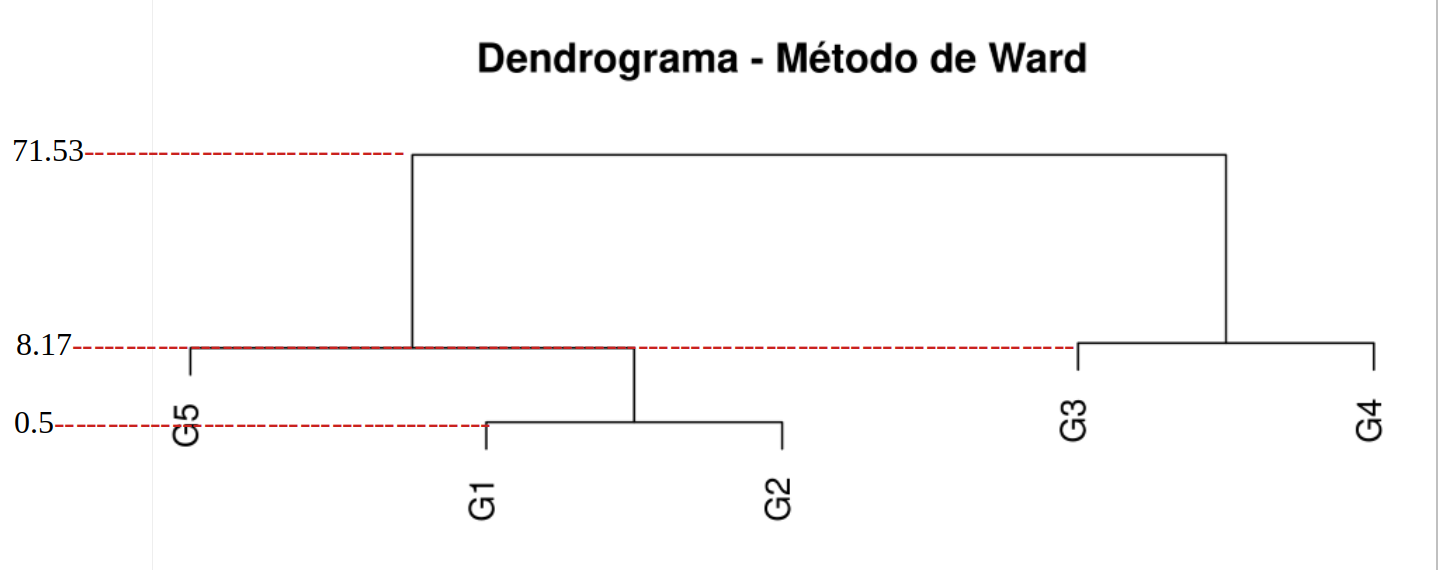
\includegraphics[width=0.8\textwidth]{../img/dendrograma.png}
        \caption{Dendrograma resultante (Fuente: elaboración propia).}
    \end{figure}

\end{ejemplo}


\subsubsection{Métodos disociativos}

Como ya apuntamos al comienzo de la subsección, un método jerárquico \textit{disociativo} comienza con un único cluster constituido por todos los individuos
de nuestro conjunto de datos y lo divide en dos clusters. Sucesivamente, en cada iteración, uno de los clusters se divide en dos subclusters hasta conseguir
un cluster por elemento. \newline

Aunque la forma de calcular la distancia entre clusters es igual que en los aglomerativos, la diferencia está en que como se parte de un único cluster, se va
a intentar maximizar las distancias o, equivalentemente, minimizar las similitudes. En definitiva, lo que se persigue es separar los elementos más disímiles en 
clusters diferentes. \newline

Los métodos disociativos son generalmente de dos clases: \textit{monotéticos} y \textit{politéticos}. En un enfoque monotético, la división de un grupo en dos 
subgrupos se basa en una sola variable y resultan útiles cuando las variables son de tipo binario, mientras que el enfoque politético utiliza las $p$ 
variables para realizar la división. \newline

Tienen la misma desventaja que los aglomerativos: una vez realizada la partición, un elemento no puede trasladarse a otro grupo al que no pertenece en el momento 
de la partición. En cambio, si se buscan grupos más grandes, a veces se prefiere el enfoque disociativo al aglomerativo, en el que los grupos más grandes se alcanzan
solo tras un gran número de uniones de grupos más pequeños. A pesar de esto, son métodos mucho menos conocidos que los aglomerativos, de ahí que no haya tanta 
bibliografía acerca de ellos. \newline

Un aspecto fundamental en su aplicación es determinar el momento adecuado para parar la subdivisión de un cluster y empezar a fragmentar otro. Esto lo resuelve la 
variante del método propuesta por MacNaughton-Smith en el año 1964, diseñada especialmente para medidas de asociación positivas, y que presentamos formalmente
a continuación: \newline

Sea $C$ un cluster inicial. Definimos un subconjunto $S \subset C$ como el grupo fragmentado, y su complemento $R = C\backslash S$ como el resto del cluster. El 
proceso de división consistirá en evaluar, para cada elemento $x \in R$, la diferencia entre su disimilaridad promedio con los elementos de $R$ y su disimilaridad 
promedio con los elementos de $S$. \newline

La distancia promedio de un elemento $x$ respecto a un conjunto $A$ viene dada por: 
\[
d(x,A) = \frac{1}{n_{A}} \sum_{y\in A} d(x,y)
\]

donde $d(x,y)$ represeta la medida de disimilaridad entre los elementos $x$ e $y$.\newline

Para cada $x\in R$, calculamos:
\[
\Delta (x) = d(x,R) - d(x,S)
\]

Si existe un $x^{'} \in R$ tal que $\max_{x \in R}{\Delta (x)} > 0$, entonces $x^{'}$ se traslada a $S$. En caso contrario, el procedimiento se detiene y la división
se completa. \newline

\begin{nota}
    Podemos inicalizar el conjunto fragmentado $S$ con el elemento $x_{0} \in C$ que tenga la mayor disimilaridad promedio respecto a los demás elementos del cluster.
\end{nota}

%Para dividir un cluster, trabajamos con un grupo fragmentado y el resto. Buscamos el elemento del resto cuya distancia promedio (disimilaridad) con respecto a los demás
%elementos del resto, menos su distancia promedio con respecto a los elementos del grupo fragmentado sea mayor. Si la mayor diferenca es positiva, el elemento se
%traslada al grupo fragmentado. Si la mayor diferencia es negativa, el procedimiento se detiene y la división se completa. Podemos comenzar el grupo fragmentado con
%el elemento que tenga la mayor distancia promediio con respecto a los demás elementos del grupo.


\subsection{Métodos no jerárquicos} %Bib-1, Bib-2, Bejar-AC

La información recogida en esta subsección y en las sucesivas subsubsecciones se ha obtenido principalmente de las fuentes biliográficas \cite{Bib-1, bejar-AC, Bib-2}.

Los \textit{métodos no jerárquicos} para el análisis cluster, también conocidos como métodos de partición, simplemente dividen los datos en un número predeterminado $k$
de clusters, donde no existe una relación jerárquica entre la solución con $k$ clusters y la de $(k+1)$, es decir, la solución con $k$ clusters no es el paso previo para
la solución con $(k+1)$. Esta es la principal diferencia con respecto a los jerárquicos, donde el número de clusters era desconocido a priori. \newline

En definitiva, dado un número $k$, buscamos particionar los datos en $k$ clusters de modo que los elementos dentro de cada cluster sean similares entre sí, mientras que los elementos 
de clusters distintos sean bastante diferentes.\newline

Se caracterizan por tener una estructura plana, es decir, no implican la construcción de una estructura jerárquica en forma de árbol, a diferencia de los métodos jerárquicos.
En su lugar, los elementos se asignan a los clusters directamente, teniendo en cuenta el número predefinido de clusters, $k$. No se sigue un proceso progresivo de combinación
o separación de grupos, como ocurre en los jerárquicos. \newline

\begin{nota}
    Los algoritmos no jerárquicos son mucho más eficientes que los jerárquicos en términos computacionales.
\end{nota}

\subsubsection{Método \textit{k-means}}

El algoritmo \textit{k-means}, propuesto por MacQueen en el año 1967, es el método más popular entre los no jerárquicos. Debido a su extrema eficiencia, se usa con frecuencia en proyectos de
grandes dimensiones. Se denomina \textit{k-means} (k-medias) porque asigna cada individuo al cluster cuyo centroide esté más próximo, de entre $k$ clusters prefijados. Dicho centroide se calcula 
a partir de los elementos que conforman el cluster después de cada asignación, en lugar de hacerlo al final de cada ciclo, como ocurre en otros métodos, lo cual es un aspecto
clave de este algoritmo. \newline
Cabe resaltar que este algoritmo necesita acceso a los datos originales y permite mover los elementos de un cluster a otro, una reasignación que no está disponible en los métodos 
jerárquicos. \newline

Veamos cómo funciona el algoritmo: \newline

Sea $\mathcal{L} = \{x_{i} / i = 1,\dots,n\}$ el conjunto de puntos que conforman nuestro conjunto de datos y sea $k$ el número de clusters. Elegimos $k$ elementos que nos servirán de 
\textit{semillas}, las cuales se reemplazarán por los centroides de los clusters en el transcurso del algoritmo. Hay varias formas de elegir dichas semillas:
\begin{itemize}
    \item[(1)] Seleccionando $k$ elementos al azar, aunque quizás separados por una mínima distancia.
    \item[(2)] Eligiendo los $k$ primeros elementos del conjunto de datos, sujetos a una distancia mínima. 
    \item[(3)] Seleccionando los $k$ puntos más alejados entre sí en base a una medida de disimilaridad.   
\end{itemize}

entre otras opciones. \newline

Una vez elegidas las semillas, cada elemento de nuestro conjunto de datos se asignará al cluster que tenga la semilla más cercana, en términos de distancia euclidea. Una vez que 
un cluster pase a tener más de un elemento, se reemplaza la semilla por su centroide. Cuando todos los elementos hayan sido asignados, entonces nos plantemos si cada elemento está
más cerca del centroide del cluster donde está asignado o del de otro cluster. Esto es, calculamos el Error Cuadrático Medio (ECM) de cada observación con respecto al
centroide de su clúster actual y el resto de centroides:
\[
ECM = \sum_{j=1}^{k}\sum_{i_{C_{j}}}(x_{i_{C_{j}}}-\bar{x}_{j})^{'}(x_{i_{C_{j}}}-\bar{x}_{j})
\]

donde $\bar{x}_{j}$ es el centroide del $j$-ésimo cluster y $C_{j}$ es el cluster que contiene a $x_{i_{C_{j}}}$. \newline

Si está más cerca del centroide de otro cluster, dicho elemento se traslada a dicho cluster y se recalculan los centroides de ambos. El proceso continúa hasta 
que no se puedan hacer más mejoras en términos de error cuadrátrico medio (se persigue minimizar el ECM). \newline

Cabe destacar que este método es bastante sensible a la elección de las semillas al comienzo del mismo. Se aconseja probar con distintas semillas y analizar los resultados: si 
con diferentes elecciones de semillas se dan resultados muy diferentes, o se requieren demasiadas iteraciones para estabilizarse (convergencia lenta), podemos sospechar que los datos no 
forman grupos bien dfinidos de forma natural. \newline

También puede usarse como mejora de los métodos jerárquicos: se agrupan primero los elementos mediante un método jerárquico y luego, utilizando como semillas los centroides de estos grupos
aplicamos el algoritmo. De esta forma, podremos reasignar los puntos de un cluster a otro, en caso de necesitarlo. Suplimos así el handicap de los aglomerativos. \newline

Ofrecemos a continuación un ejemplo con el que ilustraremos el funcionamiento del método. Este ejemplo es de elaboración propia, aunque basado en el ejemplo ilustrativo del método 
$k$-means recogido en la fuente bibliográfica \cite{quesada-tfg}.

\begin{ejemplo}
    Supongamos que tenemos $8$ genotipos, $G_{1}, G_{2},\dots,G_{8}$, sobre los que observamos la expresión de dos genes, $A$ y $B$:

    \begin{table}[h]
        \centering
        \begin{tabular}{|c|c|c|}
            \hline
            \textbf{Genotipo} & \textbf{$A$} & \textbf{$B$} \\
            \hline
            $G_{1}$ & 2.5 & 2.7 \\
            \hline
            $G_{2}$ & 5.1 & 4.9 \\
            \hline
            $G_{3}$ & 2.8 & 3.2 \\
            \hline
            $G_{4}$ & 3.0 & 2.4 \\
            \hline
            $G_{5}$ & 8.3 & 3.3 \\
            \hline
            $G_{6}$ & 4.6 & 6.1 \\
            \hline
            $G_{7}$ & 9.3 & 4.6 \\
            \hline
            $G_{8}$ & 5.3 & 3.8\\
            \hline
            
        \end{tabular}
        \caption{Ejemplo método \textit{$k$-means}}

    \end{table}

    Queremos aplicar el método no jerárquico $k$-means para $k=3$. \newline

    Comenzamos eligiendo por semillas $3$ elementos aleatorios, $g_{i} = (a_{i},b_{i})$, $i=1,\dots,8$, de entre nuestro conjunto de datos. Estos
    serán los primeros centroides:
    \[
    \bar{g}_{C_{1}} = (3.0,2.4) \hspace{0.3cm} \bar{g}_{C_{2}} = (8.3,3.3) \hspace{0.3cm} \bar{g}_{C_{3}} = (4.6,6.1)
    \]

    Calculamos las distancias de todos los puntos de nuestro dataset a estos centroides y obtenemos:

    \begin{table}[h]
        \centering
        \begin{tabular}{|c|c|c|c|c|}
            \hline
            \textbf{$g_{i}$} & \textbf{$C_{1}$} & \textbf{$C_{2}$} & \textbf{$C_{3}$} & \textbf{Cluster más cercano}\\
            \hline
            $g_{1}$ & $0.5830952$ & $5.830952$ & $3.996248$ & $C_{1}$\\
            \hline
            $g_{2}$ & $3.2649655$ & $3.577709$  & $1.300000$ & $C_{3}$\\
            \hline
            $g_{3}$ & $0.8246211$ & $5.500909$ & $3.413210$ & $C_{1}$\\
            \hline
            $g_{4}$ & $0.0000000$ & $5.375872$ & $4.031129$ & $C_{1}$\\
            \hline
            $g_{5}$ & $5.3758720$ & $0.000000$ & $4.640043$ & $C_{2}$\\
            \hline
            $G_{6}$ & $4.0311289$ & $4.640043$ & $0.000000$ & $C_{3}$\\
            \hline
            $G_{7}$ & $6.6730802$ & $1.640122$ & $4.933559$ & $C_{2}$\\
            \hline
            $G_{8}$ & $2.6925824$ & $3.041381$ & $2.404163$ & $C_{3}$ \\
            \hline
            
        \end{tabular}
        \caption{Cálculo distancias respecto centroides}

    \end{table}

    A continuación, como todos los clusters han pasado de tener más de un elemento,$C_{1} = \{g_{1},g_{3},g_{4}\}$,
    $C_{2} = \{g_{5},g_{7}\}$, $C_{3} = \{g_{2},g_{6},g_{8}\}$, recalculamos los centroides:

    \[
    \bar{g}_{C_{1}} = (2.767,2.767) \hspace{0.3cm} \bar{g}_{C_{2}} = (8.80,3.95) \hspace{0.3cm} \bar{g}_{C_{3}} = (5.0,4.9333)
    \]

    Calculamos de nuevo las distancias de cada punto a los nuevos centroies para ver si hay que hacer alguna reasignación de algún punto
    a otro cluster:

    \begin{table}[h]
        \centering
        \begin{tabular}{|c|c|c|c|c|}
            \hline
            \textbf{$g_{i}$} & \textbf{$C_{1}$} & \textbf{$C_{2}$} & \textbf{$C_{3}$} & \textbf{Cluster más cercano}\\
            \hline
            $g_{1}$ & $0.2748737$ & $6.422811$ & $3.3522573$ & $C_{1}$\\
            \hline
            $g_{2}$ & $3.1615749$ & $3.820013$  & $0.1053987$ & $C_{3}$\\
            \hline
            $g_{3}$ & $0.4346136$ & $6.046693$ & $2.8007729$ & $C_{1}$\\
            \hline
            $g_{4}$ & $0.4346134$ & $6.003541$ & $3.2276321$ & $C_{1}$\\
            \hline
            $g_{5}$ & $5.5589767$ & $0.820061$ & $3.6820740$ & $C_{2}$\\
            \hline
            $G_{6}$ & $3.8042375$ & $4.718315$ & $1.2333649$ & $C_{3}$\\
            \hline
            $G_{7}$ & $6.7856876$ & $0.820061$ & $4.3128980$ & $C_{2}$\\
            \hline
            $G_{8}$ & $2.7359744$ & $3.503213$ & $1.1723348$ & $C_{3}$ \\
            \hline
            
        \end{tabular}
        \caption{Cálculo distancias respecto centroides}

    \end{table}

    Observamos que la asignación de puntos a clusters se mantiene constante con respecto al paso previo. Esto quiere decir que no es necesaria ninguna
    reasignación y, por tanto, que las asignaciones son definitivas. La agrupación la podemos ver en la figura 3.4.

    \begin{figure}[h]
        \centering
        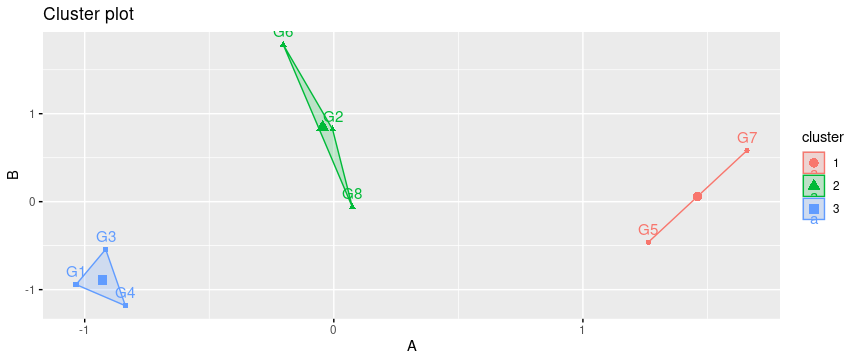
\includegraphics[width=0.8\textwidth]{../img/kmeans.png}
        \caption{Gráfico resultado final k-means. (Fuente: elaboración propia).}
    \end{figure}
    
    
\end{ejemplo}

Por último, supongamos que hay elementos en nuestro conjunto de datos que podríamos catalogar como \textit{atípicos}, es decir, supongamos que tenemos \textit{outliers}. Estos valores, al 
ser muy dispares respecto a los demás, van a tener una gran influencia en el cálculo de los centroides, lo cual va a condicionar la agrupación. Esto lo podemos solucionar con el 
método $k$-medoids, que presentamos a continuación.

\subsubsection{Método \textit{$k$-medoids}}

El algoritmo \textit{$k$-medoids} se propone como una variante del método $k$-means que es mucho más robusta a ruidos y outliers. En lugar de 
usar el centroide como centro de un grupo, este algoritmo usa un punto real del grupo para representarlo; el \textit{medoide}, que es el objeto ubicado
más centralmennte en el grupo, y que minimiza la suma de disimilaridades respecto a los demás puntos, en lugar de la suma de los cuadrados de las distancias Euclideas \cite{kmedoids}. Aquí es donde
se refleja la robustez del método ante datos anómalos como los outliers. Pese a las ventajas evidentes que tiene el método, se ha visto que para conjuntos de 
datos muy grandes, la eficiencia del método se ve disminuida. \newline

El algoritmo comienza con la matriz de proximidad $D = (d_{ij})$, donde $d_{ij} = d(x_{i},x_{j})$, con $d$ una medida de disimilaridad, que nos la pueden dar de antemano o
bien la podemos calcular a partir del conjunto de datos, y una configuración inicial de los elementos en $k$ clusters. Usando la matriz $D$, podemos encontrar el elemento de 
cada cluster que minimiza la disimilaridad total con respecto a todos los elementos de su cluster (el medoide). Esto es, dado un cluster $C_{m}$, $m\in\{1,\dots,k\}$, se busca encontrar
un elemento $\bar{x}_{m}$ que haga mínima la suma $\sum_{i_{C_{m}}}d_(x_{i_{C_{m}}},\bar{x}_{m})$. \newline

Una vez hallados los medoides de los $k$ clusters, observamos la distancia de cada punto a los distintos medoides. Si existe un cluster $j$ de entre los $k$ que había prefijados que 
tiene algún elemento $x_{j}$ que está más cerca de otro medoide, entonces este elemento se reasigna al cluster de dicho medoide. Esta reasignación favorece a la minimización de la función
objetivo:
\[
d_{medoid} = \sum_{j=1}^{k}\sum_{i_{C_{j}}}d_(x_{i_{C_{j}}},\bar{x}_{j})
\]

A continuación se relocalizan medoides y se vuelven a reasignar los elementos. Se repite el proceso hasta que no haya reasignaciones que reduzcan 
el valor de la función objetivo.



\subsubsection{Determinación del número de clusters óptimo}

Los métodos no jerárquicos agrupan los datos en un número prefijado de clusters, $k$. Hay varios métodos para determinar
dicho número clusters de forma óptima. A continuación describimos tres de los métodos más usados: el \textit{método de Elbow} y el \textit{método de Silhouette}. \newline

\textit{Método de Elbow} \newline

Teniendo en cuenta que el objetivo que se persigue a la hora de agrupar los datos en $k$ clusters es obtener dichos cluster de forma que se minimice la varianza total intra-clusters (wss), es decir,
la suma de los errores cuadráticos para cada $k$, podemos determinar el número de clusters óptimo de la siguiente forma: \newline

Para distintos valores de $k$ $ (k = 1,2,\dots,10,\dots,15,\dots)$ aplicamos un algoritmo de clustering. Para cada número de clusters con el que hemos probado el algoritmo, calculamos la varianza
total intra-clusters. Obtenemos así una serie de puntos $ (k_{i}$,$wss_{k_{i}})$, cluster-wss. Graficando dichos puntos, obtenemos una curva de la wss en función del número de clusters, $k$. \newline

El punto en el que la curva presente un `codo', se considera indicador del número de clusters óptimo. Este punto es justo aquel en el que las varianzas intra-clusters pasan de disminuir rápidamente
a empezar a disminuir de forma lineal conforme aumenta el número de clusters. \newline

\begin{ejemplo}
    Si aplicamos este método al ejemplo de los genotipos usado para ilustrar el método $k$-means, obtenemos la siguente curva:
    \begin{figure}[h]
        \centering
        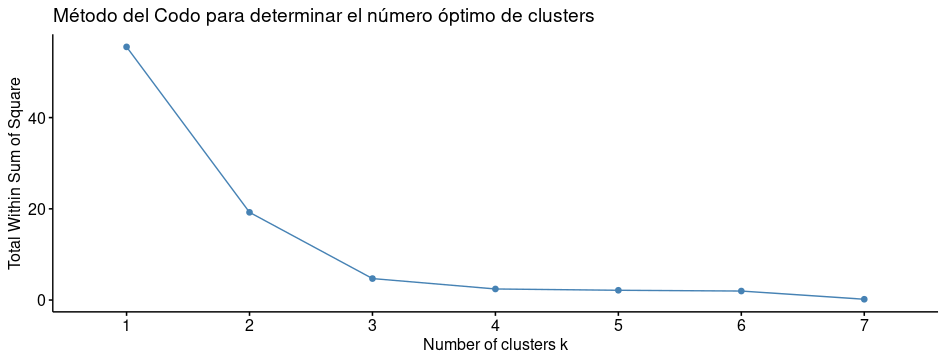
\includegraphics[width=0.8\textwidth]{../img/elbow.png}
        \caption{Método de Elbow aplicado al ejemplo del método k-means (Fuente: elaboración propia).}
    \end{figure}

    Observamos que el codo está n $k=3$, justo el número de clusters que habíamos prefijado para aplicar el método $k$-means. Por tanto, fuimos bastante acertados.
    
\end{ejemplo}

\textit{Método de la Silueta} \newline  %referencia bejar y bib-2

Este enfoque para la determinación del número óptimo de clusters, también conocido como \textit{silueta promedio}, mide la calidad de un cluster, es decir, cómo de adecuado es un objeto dentro de un cluster o,
equivalentemente, cómo de bien están separados los clusters. De acuerdo con este método, el número óptimo de clusters, $k$, vendrá dado por el valor $k$ que maximice la silueta promedio, la cual se calcula de
la forma que presentamos a continuación:

Supongamos que nos dan una partición de nuestro conjunto de datos en $k$ clusters, $\mathcal{C_{k}}$. Sea $C_{i}$ el cluster que contiene al $i$-ésimo elemento. Sea $a_{i}$ la distancia promedio del $i$-ésimo elemento al resto de 
objetos del mismo cluster $C_{i}$. Sea tambén $C_{j}$ otro cluster, con $j \neq i$, y consideremos la distancia promedo del $i$-ésimo elemento a todos los de $C_{j}$, $d(i,C_{j})$. Calculamos a continuación $d(i,C_{j})$,
para todos los clusters distintos de $C_{i}$. Sea entonces el mínimo de dichas distancas, $b_{i} = \min_{C_{j}\neq C_{i}}d(i,C_{j})$. El $i$-ésimo valor de silueta promedio viene dado por:
\[
s_{i}(\mathcal{C}_{k}) = s_{ik} = \frac{b_{i}-a_{i}}{\max (a_{i},b_{i})}
\]

de manera que $s_{ik} \in [-1,1]$.\newline

Haciendo el promedio de las siluetas promedio para cada punto del conjunto de datos, obtenemos la \textit{silueta promedio}, $\bar{s}_{k}$. Calculando esta silueta promedio para distintos valor de $k$, obtenemos una serie de 
puntos $ (k,\bar{s}_{k})$ que podremos representar. El valor de $k$ para el cual $\bar{s}_{k}$ sea máximo, determina el número óptimo de clusters. \newline

\begin{ejemplo}
    Si aplicamos este método al ejemplo de los genotipos usado para ilustrar el método $k$-means, obtenemos la siguente gráfica de puntos $(k,\bar{s}_{k})$:
    \begin{figure}[h]
        \centering
        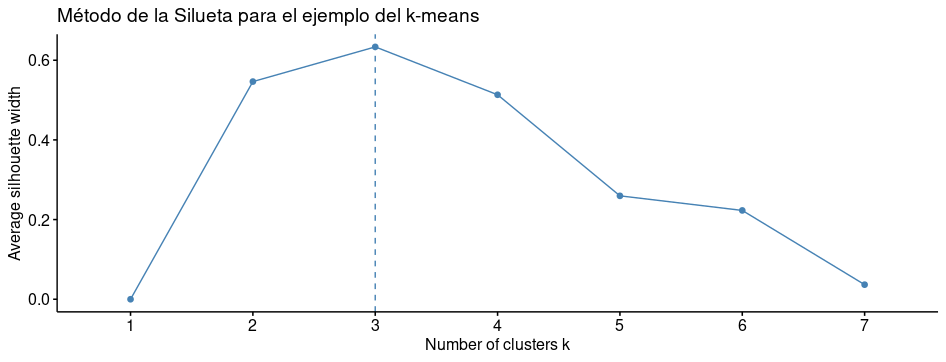
\includegraphics[width=0.8\textwidth]{../img/silueta.png}
        \caption{Método de la Silueta aplicado al ejemplo del método k-means (Fuente: elaboración propia).}
    \end{figure}

    Observamos que el máximo de la silueta promedio se alcanza en $k=3$, como era de esperar.
\end{ejemplo}